%File: anonymous-submission-latex-2026.tex
\documentclass[letterpaper]{article} % DO NOT CHANGE THIS
\usepackage[submission]{aaai2026}  % DO NOT CHANGE THIS
\usepackage{times}  % DO NOT CHANGE THIS
\usepackage{helvet}  % DO NOT CHANGE THIS
\usepackage{courier}  % DO NOT CHANGE THIS
\usepackage[hyphens]{url}  % DO NOT CHANGE THIS
\usepackage{graphicx} % DO NOT CHANGE THIS
\urlstyle{rm} % DO NOT CHANGE THIS
\def\UrlFont{\rm}  % DO NOT CHANGE THIS
\usepackage{natbib}  % DO NOT CHANGE THIS AND DO NOT ADD ANY OPTIONS TO IT
\usepackage{caption} % DO NOT CHANGE THIS AND DO NOT ADD ANY OPTIONS TO IT
\frenchspacing  % DO NOT CHANGE THIS
\setlength{\pdfpagewidth}{8.5in} % DO NOT CHANGE THIS
\setlength{\pdfpageheight}{11in} % DO NOT CHANGE THIS
%
% These are recommended to typeset algorithms but not required. See the subsubsection on algorithms. Remove them if you don't have algorithms in your paper.
\usepackage{algorithm}
\usepackage{algorithmic}

%
% These are are recommended to typeset listings but not required. See the subsubsection on listing. Remove this block if you don't have listings in your paper.
\usepackage{newfloat}
\usepackage{listings}
\DeclareCaptionStyle{ruled}{labelfont=normalfont,labelsep=colon,strut=off} % DO NOT CHANGE THIS
\lstset{%
	basicstyle={\footnotesize\ttfamily},% footnotesize acceptable for monospace
	numbers=left,numberstyle=\footnotesize,xleftmargin=2em,% show line numbers, remove this entire line if you don't want the numbers.
	aboveskip=0pt,belowskip=0pt,%
	showstringspaces=false,tabsize=2,breaklines=true}
\floatstyle{ruled}
\newfloat{listing}{tb}{lst}{}
\floatname{listing}{Listing}
%
% Keep the \pdfinfo as shown here. There's no need
% for you to add the /Title and /Author tags.
\pdfinfo{
/TemplateVersion (2026.1)
}
\definecolor{LAMPYellow}{RGB}{255,220,112}
\definecolor{HeaderGray}{RGB}{235,235,235}
\definecolor{AvgBlue}{RGB}{226,241,255}
\definecolor{GainGreen}{RGB}{32,132,84}
\definecolor{DropRed}{RGB}{190,54,54}
\newcommand{\tblhead}[1]{\strut #1}
\newcommand{\lampcell}[1]{\begingroup\setlength{\fboxsep}{0pt}\colorbox{LAMPYellow}{\makebox[6.7em][c]{\rule[-1.12ex]{0pt}{4.45ex}\bfseries\boldmath #1}}\endgroup}
\newcommand{\avgcell}[1]{\begingroup\def\avgcontent{#1}\def\avgheader{Avg}\ifx\avgcontent\avgheader\bfseries #1\else\setlength{\fboxsep}{0pt}\colorbox{AvgBlue}{\makebox[3.55em][c]{\strut #1}}\fi\endgroup}
\newcommand{\metriclampcell}[1]{\begingroup\setlength{\fboxsep}{0pt}\colorbox{LAMPYellow}{\makebox[7.05em][c]{\rule[-0.96ex]{0pt}{3.95ex}\bfseries\boldmath #1}}\endgroup}
\newcommand{\lampband}{\noalign{\begingroup\color{LAMPYellow}\hrule height 3.35ex\endgroup\kern-3.35ex}}
\newcommand{\headband}{\noalign{\begingroup\color{HeaderGray}\hrule height 6.15ex\endgroup\kern-6.15ex}}
\newcommand{\gainup}[1]{\makebox[5.85em][l]{\textcolor{GainGreen}{\(\uparrow\)#1}}}
\newcommand{\gaindown}[1]{\makebox[5.85em][l]{\textcolor{GainGreen}{\(\downarrow\)#1}}}
\newcommand{\dropdown}[1]{\makebox[5.85em][l]{\textcolor{DropRed}{\(\downarrow\)#1}}}
\newcommand{\neutraldelta}[1]{\makebox[5.85em][l]{\textcolor{GainGreen}{#1}}}

% DISALLOWED PACKAGES
% \usepackage{authblk} -- This package is specifically forbidden
% \usepackage{balance} -- This package is specifically forbidden
% \usepackage{color (if used in text)
% \usepackage{CJK} -- This package is specifically forbidden
% \usepackage{float} -- This package is specifically forbidden
% \usepackage{flushend} -- This package is specifically forbidden
% \usepackage{fontenc} -- This package is specifically forbidden
% \usepackage{fullpage} -- This package is specifically forbidden
% \usepackage{geometry} -- This package is specifically forbidden
% \usepackage{grffile} -- This package is specifically forbidden
% \usepackage{hyperref} -- This package is specifically forbidden
% \usepackage{navigator} -- This package is specifically forbidden
% (or any other package that embeds links such as navigator or hyperref)
% \indentfirst} -- This package is specifically forbidden
% \layout} -- This package is specifically forbidden
% \multicol} -- This package is specifically forbidden
% \nameref} -- This package is specifically forbidden
% \usepackage{savetrees} -- This package is specifically forbidden
% \usepackage{setspace} -- This package is specifically forbidden
% \usepackage{stfloats} -- This package is specifically forbidden
% \usepackage{tabu} -- This package is specifically forbidden
% \usepackage{titlesec} -- This package is specifically forbidden
% \usepackage{tocbibind} -- This package is specifically forbidden
% \usepackage{ulem} -- This package is specifically forbidden
% \usepackage{wrapfig} -- This package is specifically forbidden
% DISALLOWED COMMANDS
% \nocopyright -- Your paper will not be published if you use this command
% \addtolength -- This command may not be used
% \balance -- This command may not be used
% \baselinestretch -- Your paper will not be published if you use this command
% \clearpage -- No page breaks of any kind may be used for the final version of your paper
% \columnsep -- This command may not be used
% \newpage -- No page breaks of any kind may be used for the final version of your paper
% \pagebreak -- No page breaks of any kind may be used for the final version of your paperr
% \pagestyle -- This command may not be used
% \tiny -- This is not an acceptable font size.
% \vspace{- -- No negative value may be used in proximity of a caption, figure, table, section, subsection, subsubsection, or reference
% \vskip{- -- No negative value may be used to alter spacing above or below a caption, figure, table, section, subsection, subsubsection, or reference

\setcounter{secnumdepth}{0} %May be changed to 1 or 2 if section numbers are desired.

% The file aaai2026.sty is the style file for AAAI Press
% proceedings, working notes, and technical reports.
%

% Title

% Your title must be in mixed case, not sentence case.
% That means all verbs (including short verbs like be, is, using,and go),
% nouns, adverbs, adjectives should be capitalized, including both words in hyphenated terms, while
% articles, conjunctions, and prepositions are lower case unless they
% directly follow a colon or long dash

% LAMP-Merge：面向单次异步临床模型的长尾感知医学原型融合。
\title{LAMP-Merge: Long-tail-Aware Medical Prototype Merging for One-shot Asynchronous Clinical Models}
\author{
    %Authors
    % All authors must be in the same font size and format.
    Written by AAAI Press Staff\textsuperscript{\rm 1}\thanks{With help from the AAAI Publications Committee.}\\
    AAAI Style Contributions by Pater Patel Schneider,
    Sunil Issar,\\
    J. Scott Penberthy,
    George Ferguson,
    Hans Guesgen,
    Francisco Cruz\equalcontrib,
    Marc Pujol-Gonzalez\equalcontrib
}
\affiliations{
    %Afiliations
    \textsuperscript{\rm 1}Association for the Advancement of Artificial Intelligence\\
    % If you have multiple authors and multiple affiliations
    % use superscripts in text and roman font to identify them.
    % For example,

    % Sunil Issar\textsuperscript{\rm 2},
    % J. Scott Penberthy\textsuperscript{\rm 3},
    % George Ferguson\textsuperscript{\rm 4},
    % Hans Guesgen\textsuperscript{\rm 5}
    % Note that the comma should be placed after the superscript

    1101 Pennsylvania Ave, NW Suite 300\\
    Washington, DC 20004 USA\\
    % email address must be in roman text type, not monospace or sans serif
    proceedings-questions@aaai.org
%
% See more examples next
}

%Example, Single Author, ->> remove \iffalse,\fi and place them surrounding AAAI title to use it
\iffalse
\title{My Publication Title --- Single Author}
\author {
    Author Name
}
\affiliations{
    Affiliation\\
    Affiliation Line 2\\
    name@example.com
}
\fi

\iffalse
%Example, Multiple Authors, ->> remove \iffalse,\fi and place them surrounding AAAI title to use it
\title{My Publication Title --- Multiple Authors}
\author {
    % Authors
    First Author Name\textsuperscript{\rm 1},
    Second Author Name\textsuperscript{\rm 2},
    Third Author Name\textsuperscript{\rm 1}
}
\affiliations {
    % Affiliations
    \textsuperscript{\rm 1}Affiliation 1\\
    \textsuperscript{\rm 2}Affiliation 2\\
    firstAuthor@affiliation1.com, secondAuthor@affilation2.com, thirdAuthor@affiliation1.com
}
\fi


% REMOVE THIS: bibentry
% This is only needed to show inline citations in the guidelines document. You should not need it and can safely delete it.
\usepackage{bibentry}
% END REMOVE bibentry

\begin{document}

\maketitle

\begin{abstract}
%
% 多中心医学模型通常在具有不同设备、不同患者群体和不同诊断标签覆盖范围的医院之间异步训练。本文研究单次异步医学模型融合问题：每个客户端在本地训练后只上传一次，服务器在不访问原始医学图像且不进行联邦优化轮次的条件下构建全局模型。我们将聚合诱导的预测坍缩识别为通用模型融合方法的核心失效模式。研究进一步表明，由于长尾医学先验会使多数类坍缩在准确率上呈现出具有迷惑性的竞争力，原始准确率可能掩盖这一失效。为此，我们提出 LAMP-Merge，即一种长尾感知的医学原型融合框架，它根据客户端侧类别统计重建诊断原型头，并用有界先验偏置校准长尾患病率。在五个医学数据集、四类视觉模型、三种客户端数量和三种非独立同分布偏斜水平上，LAMP-Merge 在 60 个客户端平均单元中的 57 个单元达到或并列超过最强非 LAMP 基线，同时提升了平衡准确率、宏 F1 和预测坍缩诊断指标。
Multicenter medical models are typically trained asynchronously across hospitals with heterogeneous acquisition devices, patient populations, and diagnostic-label coverage. We study single-shot asynchronous medical model merging, where each client uploads its locally trained model only once and the server constructs a global model without accessing raw medical images or conducting federated optimization rounds. We identify aggregation-induced prediction collapse as the central failure mode of general-purpose model-merging methods. Furthermore, we show that long-tailed medical priors can make majority-class collapse deceptively competitive in terms of raw accuracy, thereby masking this failure. To address this issue, we propose LAMP-Merge, a long-tail-aware medical prototype-merging framework that reconstructs a diagnostic prototype head from client-side class statistics and calibrates long-tail prevalence using a bounded prior bias. Across five medical datasets, four vision-model families, three client-population sizes, and three levels of non-IID skew, LAMP-Merge matches or surpasses the strongest non-LAMP baseline in 57 of 60 client-averaged settings, while improving balanced accuracy, macro-F1, and prediction-collapse diagnostic metrics.

%医学模型融合 异步融合 预测性坍缩 长尾校准 隐私保护学习
Index Terms:medical model merging, asynchronous fusion, predictive collapse, long-tail calibration, privacy-preserving learning
\end{abstract}


% Uncomment the following to link to your code, datasets, an extended version or similar.
% You must keep this block between (not within) the abstract and the main body of the paper.
% \begin{links}
%     \link{Code}{https://aaai.org/example/code}
%     \link{Datasets}{https://aaai.org/example/datasets}
%     \link{Extended version}{https://aaai.org/example/extended-version}
% \end{links}

\section{I Introduction}

% 医学人工智能正在从单中心模型开发走向多中心协作部署。临床诊断模型的可靠性通常依赖于跨医院、跨设备和跨患者群体的经验，因为单一机构很难同时覆盖完整疾病谱、罕见病例和不同成像条件。然而，医学数据受到伦理审批、隐私法规、设备差异和院内流程的共同限制，原始影像很难被集中到统一服务器。更现实的协作形态是：各医院在本地完成模型训练，并在训练完成后以有限的信息共享方式参与全局模型构建。
Medical artificial intelligence increasingly requires \textbf{multicenter collaboration} because no single hospital can cover the full disease spectrum, rare cases, and imaging conditions \cite{sheller2020federated,rieke2020future,kairouz2021advances}. Yet privacy requirements, device heterogeneity, and institutional workflows make \textbf{centralizing raw images impractical} \cite{kaissis2020secure,bonawitz2019towards,abadi2016deep}. A realistic alternative is for hospitals to train locally and share limited post-training information.

\begin{figure}[t]
    \centering
    
\includegraphics[width=0.96\linewidth]{figures/intro.png}
    \caption{In multicenter healthcare settings, individual clients typically observe only a subset of the global diagnostic space. Conventional parameter-level model-merging methods can therefore cause the merged global model’s predictions to concentrate on a small number of dominant classes.}
    \label{fig:intro-collapse}
\end{figure}

\begin{figure*}[t]
    \centering
    
\includegraphics[width=0.92\textwidth,height=0.34\textheight]{figures/method.png}
    \caption{Local models from multicenter hospitals typically contain only partial diagnostic knowledge, while raw medical images cannot be centrally shared. LAMP-Merge reconstructs a privacy-friendly global medical classifier through diagnostic prototype reconstruction and long-tail prevalence calibration, without accessing raw data or requiring multi-round federated optimization.}
    \label{fig_method}
\end{figure*}

% 这一现实背景产生了一个单次异步的模型融合需求。不同医院不一定同时在线，也不一定有条件在全局模型更新后反复重新训练；某些中心可能更早完成训练，某些中心可能只在固定窗口内上传模型。与此同时，服务器在部署阶段需要得到一个可供统一使用的全局诊断模型，而不是多个彼此独立、覆盖范围有限的本地模型。因此，本文研究一种模型融合场景：每个客户端只上传一次，服务器在不侵犯患者隐私(不读取客户端原始医学图像)的条件下合成一个共享检查点。
This setting requires \textbf{single-shot asynchronous model merging}. Hospitals may complete training at different times and cannot necessarily participate in repeated global updates, as assumed by conventional federated and decentralized training protocols\cite{pmlr-v54-mcmahan17a,li2020fedprox,karimireddy2020scaffold,warnat-herresthal_swarm_2021}. The server must therefore construct one deployable diagnostic model from \textbf{exactly one upload per client}, without accessing raw medical images.

% 医学图像使这一问题具有特殊难度。医院之间的差异不仅表现为图像风格或设备域偏移，还表现为诊断类别可及性的差异：一个中心可能积累了某些常见病或常规检查的大量样本，却几乎没有某些罕见诊断；另一个中心可能具有相反的病例结构。由此得到的本地模型并不是完整全局任务的独立副本，而是带有局部诊断证据的部分专家。更重要的是，医学类别分布通常呈长尾结构，多数类诊断可能占据大量样本，而少数类诊断仍然具有临床意义。一个有效的融合方法必须同时保留分散在不同客户端中的类别证据，并避免把真实长尾患病率误解释为无意义噪声。
Medical imaging makes the problem especially difficult because hospitals differ not only in device domain but also in \textbf{diagnostic-class availability} \cite{9557808,10.1371/journal.pmed.1002683,li2021fedbn}. Local models are partial experts: a client may provide strong evidence for common diagnoses while lacking rare ones. Moreover, medical labels are often \textbf{long-tailed}, so a useful merge must preserve distributed class-specific evidence while respecting genuine prevalence \cite{BUDA2018249,5597285}.

% 本文提出 LAMP-Merge，即长尾感知医学原型融合框架。其核心思想是将医学模型融合从全局参数平均问题转化为类别级诊断证据重建问题。客户端在本地使用共享参考特征提取器计算每个诊断类别的聚合原型和类别计数，并仅上传这些类别级统计及本地检查点接口。服务器随后在共享参考空间中构建全局诊断原型分类器，并在类别患病率呈现强长尾结构时引入有界的先验校准。整个过程保持单次上传，不要求服务器访问原始图像、逐样本特征、逐样本 logits 或逐样本预测。
We propose \textbf{LAMP-Merge}, a long-tail-aware medical prototype-merging framework. It recasts global parameter averaging as \textbf{class-level diagnostic-evidence reconstruction}: each client uploads class prototypes and counts computed with a shared reference extractor, and the server constructs a global prototype classifier with bounded prevalence calibration. The procedure requires one upload and never exposes raw images, per-sample features, logits, or predictions.

% 本文贡献总结如下。第一，我们提出并形式化了单次异步医学图像模型融合问题，其中客户端在本地独立训练，服务器只能使用一次上传的信息构建全局模型。第二，我们从医学诊断类别可及性和长尾患病率出发，刻画了该问题区别于一般模型融合任务的核心结构。第三，我们提出 LAMP-Merge，通过客户端侧类别原型和患病率统计重建全局诊断分类器，在保护原始图像隐私的同时缓解融合后的预测坍缩。我们在多个医学影像数据集上开展了大量实验。结果表明，无论原始数据分布情况如何，我们的LAMP-Merge均显著优于所有对比方法。此外，我们的融合方法在训练过程中无需辅助数据集或计算资源支持。
Our main contributions are as follows:
\begin{itemize}
    \item We formalize \textbf{single-shot asynchronous medical image model merging}, where independently trained clients provide one upload for global model construction.
    \item We identify \textbf{heterogeneous diagnostic-class availability and long-tailed disease prevalence} as the defining structures of this setting.
    \item We propose \textbf{LAMP-Merge}, which reconstructs a global diagnostic classifier from client-side class prototypes and prevalence statistics to mitigate prediction collapse without exposing raw images.
\end{itemize}

\section{II Related Works}

\subsection{Model Merging}

% 模型融合方法通常从参数空间、任务向量空间或几何空间整合多个检查点。权重平均和 Model Soups 直接插值模型参数；Task Arithmetic、TIES-Merging 与 DARE 处理任务增量和符号冲突；Fisher、RegMean、Model Stock、Breadcrumbs、Iso-C、FreeMerge 与 RobustMerge 进一步引入曲率、统计均值、子空间或鲁棒方向假设。然而，这些方法的核心变量仍然是全局参数、任务向量或更新方向，并不显式表示医学任务中的诊断类别证据。因此，在客户端类别覆盖不完整且患病率长尾的多中心医学图像场景中，它们容易混合“见过某类的可靠方向”和“没见过某类的缺失方向”，从而产生预测坍缩。
Model-merging methods commonly integrate checkpoints in parameter, task-vector, or geometric spaces. Weight averaging and Model Soups interpolate model parameters\cite{izmailov2018averaging,pmlr-v162-wortsman22a}; permutation-aware matching aligns hidden-unit symmetries before averaging\cite{entezari2022role,ainsworth2023gitrebasinmergingmodels}; ZipIt performs feature-level zipping across models\cite{stoica2024zipit}; Task Arithmetic, TIES-Merging, and DARE operate on task deltas and sign conflicts\cite{ilharco2023editingmodelstaskarithmetic,yadav2023tiesmergingresolvinginterferencemerging,yu2024languagemodelssupermario}; Fisher merging, RegMean, Model Stock, Breadcrumbs, Iso-C, FreeMerge, and RobustMerge further introduce curvature, mean-statistic, subspace, or robustness assumptions\cite{matena2022mergingmodelsfisherweightedaveraging,jin2025datalessknowledgefusionmerging,jang2025modelstockneedjust,davari2024modelbreadcrumbsscalingmultitask,marczak2025taskleftbehindisotropic,zheng2025freemergingfouriertransformefficient,zeng2025robustmergeparameterefficientmodelmerging}.

However, these variables are still global parameters, task vectors, or update directions rather than class-level diagnostic evidence. \textbf{They do not ask whether a client has reliable supervision for a specific medical class.} Under incomplete local class coverage and long-tailed prevalence, reliable directions from clients that observed a class can be averaged with absent or conflicting directions from clients that did not, leading to aggregation-induced prediction collapse\cite{BUDA2018249,10.1371/journal.pmed.1002683}.

\subsection{Medical Model Merging}

% 医学融合研究通常利用医学数据的领域结构，例如非规则采样时间序列、临床传感器图结构以及影像-电子病历融合。mTAN、Raindrop 和 MedFuse 表明，医学任务需要利用临床采样机制、模态异质性和患者级时间关系。然而，这些方法通常融合患者级输入或临床表征，而不是融合已经独立训练完成的图像分类器检查点；同时，它们往往需要患者样本、时间戳、多模态记录、电子病历或服务器端验证反馈。MedMerge 等训练自由医学知识迁移方法也针对视觉语言跨模态适配，而非同一任务下的单次异步检查点融合。因此，现有医学融合路线在本文约束下的核心问题是隐私与协议不匹配。
Medical fusion studies often exploit domain structures such as irregular clinical time series, physiological sensor graphs, and image-EHR fusion. mTAN, Raindrop, and MedFuse show that medical tasks benefit from modeling clinical sampling mechanisms, modality heterogeneity, and patient-level temporal relations\cite{shukla2021multitimeattentionnetworksirregularly,zhang2022graphguidednetworkirregularlysampled,hayat2023medfusemultimodalfusionclinical}.

However, these methods usually fuse patient-level inputs or clinical representations rather than independently trained image-classifier checkpoints, and they often require patient samples, timestamps, multimodal records, electronic health records, or server-side validation feedback, which conflicts with common medical privacy constraints\cite{kaissis2020secure,sheller2020federated,bonawitz2019towards}. MedMerge is a relevant training-free medical knowledge-transfer framework\cite{11382027}; however, it targets cross-modal adaptation for medical vision-language models rather than asynchronous checkpoint merging for the same classification task. \textbf{Thus, existing medical fusion routes are mismatched with our privacy and single-upload protocol constraints.} LAMP-Merge keeps the medical structure uploadable by using only class-level prototypes and prevalence counts computed locally by clients.

\subsection{Federated Learning}

% 联邦学习和去中心化学习通过通信协议完成协作训练。FedAvg 及其变体依赖多轮服务器-客户端更新；Swarm Learning 和 Gossip Learning 减弱中心化服务器角色，但仍要求参与者持续训练、交换模型并从中间模型继续优化。然而，本文研究的是训练完成后的单次异步模型融合，医院可能无法长期在线，也不能反复接收全局模型并重新训练。因此，联邦学习解决多轮协作训练问题，而 LAMP-Merge 解决单次上传后的统一模型构建问题。
Federated and decentralized learning perform collaborative training through communication protocols. FedAvg and its medical deployments rely on repeated server-client updates\cite{pmlr-v54-mcmahan17a,li2020fedprox,karimireddy2020scaffold,li2021fedbn,kaissis_secure_2020,sheller2020federated,rieke2020future,kairouz2021advances}; Swarm Learning and Gossip Learning reduce centralization but still require participants to continue training, exchanging models, and optimizing from intermediate states\cite{warnat-herresthal_swarm_2021,hegedhus_gossip_2019}.

However, our problem is single-shot asynchronous model merging after local training has finished: hospitals may not remain online, receive global checkpoints repeatedly, or run additional optimization rounds. \textbf{The limitation is therefore communication feasibility rather than only privacy.} LAMP-Merge requires one upload of a local model interface and class-level statistics, enabling the server to construct a unified diagnostic model without a multi-round feedback loop.

\section{III Method}

\begin{figure*}[t]
\centering
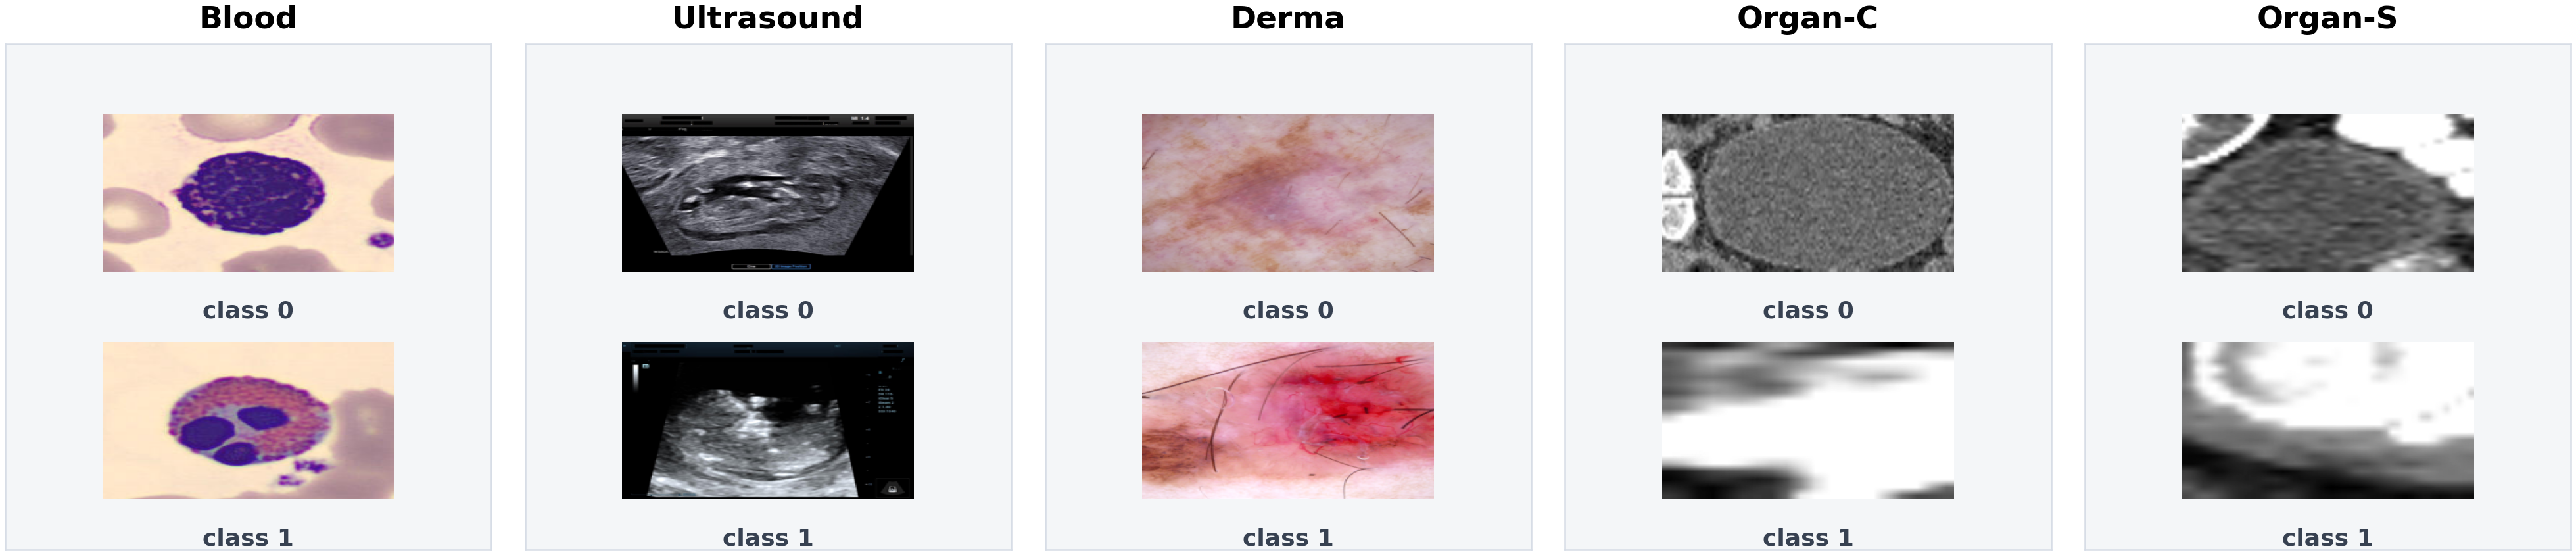
\includegraphics[width=0.96\textwidth]{figures/dataset_examples.png}
\caption{Representative training images from the five medical image datasets used in the experiments. The class IDs are shown only to illustrate category diversity within each dataset.}
\label{fig:dataset-examples}
\end{figure*}

\subsection{Motivation and Overall Idea}

% 我们发现，在局部类别覆盖的医学场景中，参数级模型融合会将多个非退化的局部预测器转化为全局坍缩预测器。而当最常见诊断类别在分布中占据很大比例时，坍缩预测器可以在缺乏真实多类别诊断能力的情况下取得较高准确率。这解释了为什么某些基线在原始准确率上依旧具有竞争力。一个有效的医学融合方法应当避免丢失罕见类别判别能力，同时在任务确实呈强长尾分布时尊重真实患病率信息。
Under partial local class coverage, parameter-level merging can turn several non-degenerate local predictors into a globally collapsed predictor. Because medical prevalence is often long-tailed, such collapse can still appear competitive in raw accuracy. A useful merger must therefore recover rare-class discrimination without discarding genuine prevalence.

% 为应对这些挑战，我们提出了MedMerge——一个基于类别级诊断原型重建的长尾感知医学模型融合框架，恢复完整诊断空间中的多类别判别方向，从结构上缓解融合后的单类或少数类预测坍缩。然而，为克服去除类别先验可能损害整体准确率的问题，我们进一步设计了长尾患病率校准模块。利用客户端上传的类别患病率计数估计全局诊断先验。具体而言，LAMP-Merge 包含两个核心组件：（1）一种用于聚合多个本地医学客户端中可靠的类别级知识，并重建不易发生坍缩的全局诊断分类器；（2）一种用于在保持多类别判别能力的同时，保留具有临床意义的多数类先验的策略。该设计实现了更加均衡且有效的诊断知识整合，使模型能够在不进行额外联邦训练、不暴露原始医学数据的条件下完成稳健的单次医学模型融合。
LAMP-Merge addresses this tension with two components. Diagnostic prototype reconstruction aggregates only class-supported evidence in a shared reference space to recover global multiclass directions. Long-tail prevalence calibration then applies a bounded prior bias estimated from client-side counts, preserving clinically meaningful majority prevalence without replacing those directions. The resulting one-shot protocol requires neither additional federated training nor raw-data exposure.

\subsection{Overview}

% LAMP-Merge 的核心框架如图所示，其核心思想是将医学模型融合从全局参数平均问题转化为类别条件诊断证据重建问题，并加以类别先验辅佐。
The core framework of LAMP-Merge is illustrated in figure\ref{fig_method}. Its central idea is to recast medical model merging from global parameter averaging into the reconstruction of class-conditional diagnostic evidence, supplemented by class-prior information.

% 值得注意的是，LAMP-Merge 并不要求服务器读取客户端原始图像，也不依赖服务器端验证集、逐样本特征或逐样本预测。客户端上传的信息仅为类别级统计量，因此该框架保持单次异步通信边界，区别于需要多轮模型下发与本地再训练的联邦学习流程。
Notably, LAMP-Merge neither requires the server to access clients’ raw images nor relies on a server-side validation set, per-sample features, or per-sample predictions. Clients upload only class-level statistics; thus, the framework preserves a single-shot asynchronous communication boundary, distinguishing it from federated learning procedures that require repeated model broadcasts and local retraining.

% 该框架由两个关键组件构成：类别级诊断原型重建模块和长尾患病率校准模块，原型重建模块用于恢复完整全局诊断空间中的多类别判别方向；随后校准模块保留合理的类别先验。
The framework comprises two key components: a class-level diagnostic prototype reconstruction module and a long-tail prevalence calibration module. The prototype reconstruction module restores multiclass discriminative directions across the complete global diagnostic space, after which the calibration module retains appropriate class-prior information.

\subsection{Diagnostic Prototype Reconstruction Module}
%假设存在 K 个医学客户端。客户端 i 拥有一个私有标注数据集 D_i={(x,y)}，该数据集来自覆盖 C 个诊断类别的类别偏斜医学分布。令 D_i,c 表示客户端 i 中属于诊断类别 c 的子集。在医学划分中，D_i,c 对许多类别都可能为空。因此，一个客户端可以对一部分诊断可靠，但对未见类别不可靠。类别无关的参数融合没有显式机制来保留这种局部可靠性结构。
Assume $K$ medical clients. Client $i$ owns a private labeled dataset $D_i=\{(x,y)\}$ drawn from a class-skewed medical distribution over $C$ diagnosis classes. Let $D_{i,c}$ denote the subset of client $i$ belonging to diagnosis class $c$. In medical partitions, $D_{i,c}$ can be empty for many classes. Thus, a client can be reliable for a subset of diagnoses but unreliable for unseen classes. A class-agnostic parameter merge has no explicit mechanism to preserve this local reliability structure.


% 因此，LAMP-Merge 首先在共享参考特征空间中重建逐类别诊断头。令 phi_0 表示在本地训练前由共享模型配置实例化得到的冻结参考骨干网络，T(.) 表示评估变换。对于每个诊断类别 c，客户端 i 计算参考空间类别原型 mu_i,c，其中 n_i,c=|D_i,c| 是类别支持数。如果 n_i,c=0，则客户端为该类别上传零支持数，并且不贡献原型证据。
Therefore, LAMP-Merge first reconstructs a class-wise diagnostic head in the shared reference feature space. Let $\phi_0$ be the frozen reference backbone instantiated from the shared model configuration before local training, and let $T(\cdot)$ be the evaluation transform. For each diagnosis class $c$, client $i$ computes a reference-space class prototype
\begin{equation}
\mu_{i,c}=\frac{1}{n_{i,c}}\sum_{(x,y)\in D_i}\mathbf{1}[y=c]\phi_0(T(x)),
\end{equation}
where $n_{i,c}=|D_{i,c}|$ is the class support count. If $n_{i,c}=0$, the client uploads zero support for that class and contributes no prototype evidence.

% 服务器将支持数转换为证据权重，其中 gamma=0.45 为默认证据指数。客户端 i 对类别 c 的归一化可靠性为 alpha_i,c。随后，全局诊断原型 p_c 由各客户端原型按照可靠性加权得到。最后，LAMP-Merge 合成一个余弦原型分类器，其中 s=20 为默认分类头缩放因子。该模块解决了当前算法的痛点：它保留了每个客户端具有证据的类别，并重建全局多类别诊断头。
The server converts support counts into evidence weights:
\begin{equation}
e_{i,c}=(n_{i,c}+1)^\gamma \mathbf{1}[n_{i,c}>0],
\end{equation}
where $\gamma=0.45$ is the default evidence exponent. The normalized reliability of client $i$ for class $c$ is
\begin{equation}
\alpha_{i,c}=\frac{e_{i,c}}{\sum_{j=1}^{K} e_{j,c}}.
\end{equation}
The global diagnosis prototype is then
\begin{equation}
p_c=\sum_{i=1}^{K}\alpha_{i,c}\mu_{i,c}.
\end{equation}
Finally, LAMP-Merge synthesizes a cosine prototype classifier:
\begin{equation}
w_c=s\frac{p_c}{\|p_c\|_2},
\end{equation}
where $s=20$ is the default head scale. This module addresses a key limitation of existing methods: it preserves the classes for which each client has supporting evidence and reconstructs a global multiclass diagnostic head.

\begin{figure*}[t]
\centering
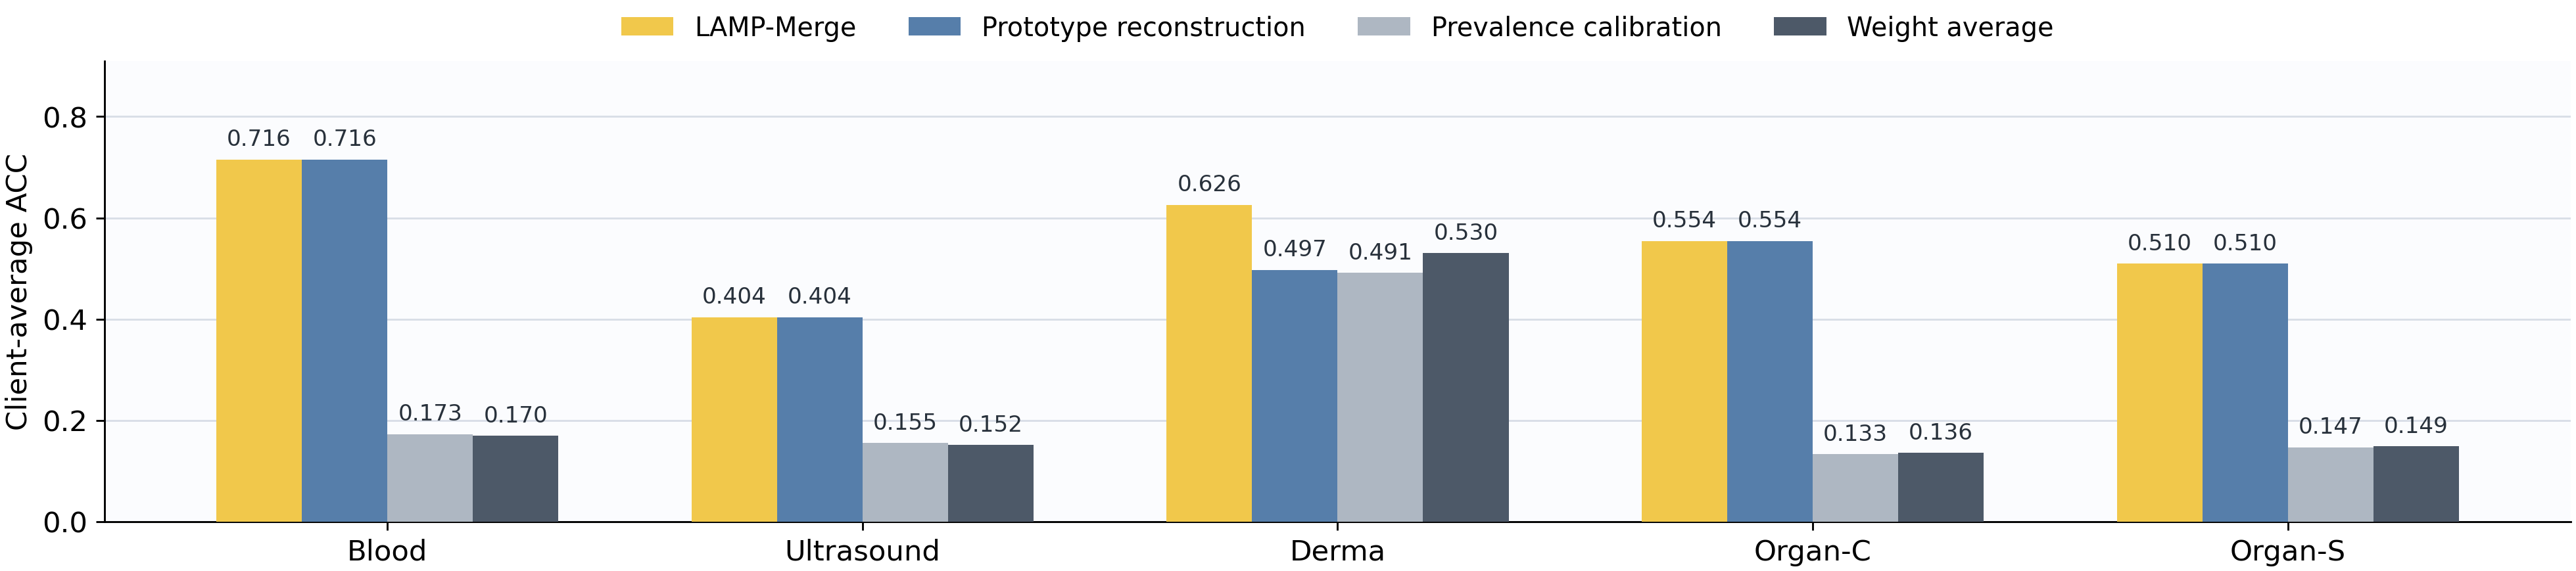
\includegraphics[width=0.92\textwidth]{figures/full_scope_module_ablation_dataset_accuracy.png}
\caption{Dataset-level client-average accuracy in the module ablation. Each bar averages 12 client-average cells from four vision-model families and three client counts; every client-average cell is computed over three Dirichlet skew levels.}
\label{fig:dataset-ablation-acc}
\end{figure*}

\begin{figure*}[t]
\centering
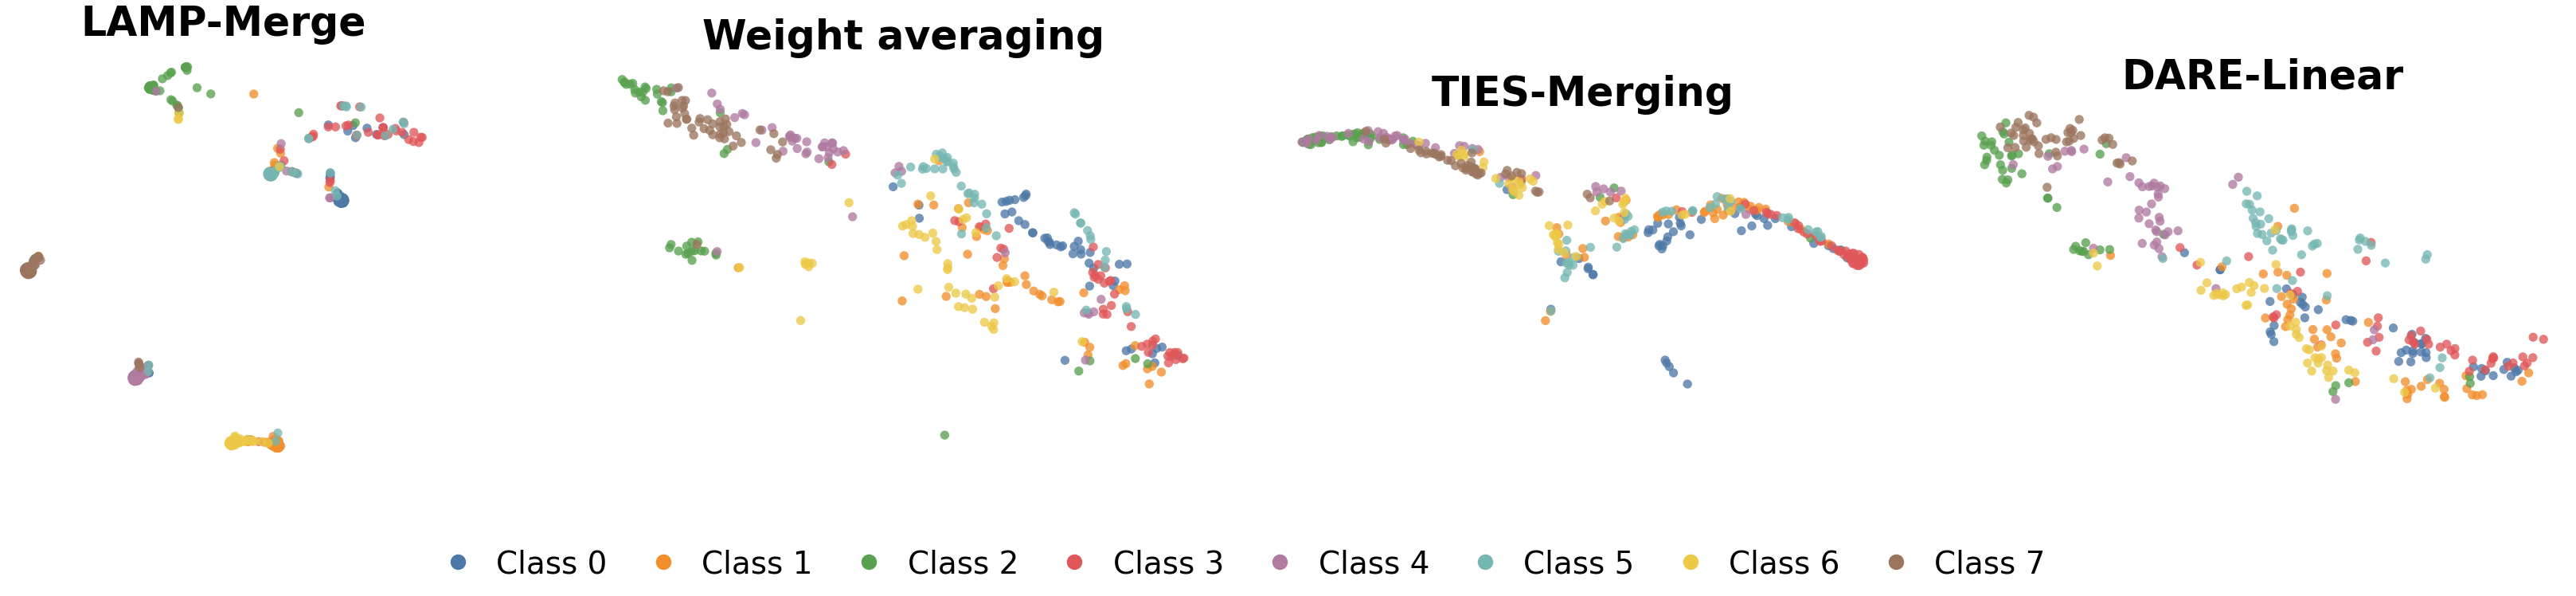
\includegraphics[width=0.98\textwidth]{figures/tsne_joint_bloodmnist_224_resnet.png}
\caption{Joint t-SNE visualization of output-probability representations on Blood. From left to right: LAMP-Merge, weight averaging, TIES-Merging, and DARE-Linear.}
\label{fig:tsne}
\end{figure*}

\subsection{Long-tail Prevalence Calibration}

% 得到这个全新的诊断头之后，为应对真实医学任务包含的长尾患病率，每个客户端还上传类别患病率计数 m_i,c。服务器据此估计全局类别先验 pi_c。我们使用 r=C max_c pi_c 度量主导类别不平衡。该模块仅在 r>tau 时激活，其中 tau=2.5 为默认值。激活后，添加一个中心化的对数先验偏置 b_c，其默认最大校准强度为 lambda=5.0。最终得分为 score_c(x)。该偏置是中心化且有界的，并附着在原型分类器上；它校准患病率，但不替代 M1 重建的多类别诊断方向。
After obtaining this newly reconstructed diagnostic head, each client additionally uploads class-prevalence counts $m_{i,c}$ to account for the long-tailed prevalence inherent in real-world medical tasks. The server estimates the global class prior
\begin{equation}
\pi_c=\frac{\sum_{i=1}^{K}m_{i,c}}{\sum_{k=1}^{C}\sum_{i=1}^{K}m_{i,k}}.
\end{equation}
We measure dominant-class imbalance by
\begin{equation}
r=C\max_c \pi_c.
\end{equation}
The module is activated only when $r>\tau$, where $\tau=2.5$ by default. When activated, it adds a centered log-prior bias
\begin{equation}
b_c=\lambda\left(\log\pi_c-\frac{1}{C}\sum_{k=1}^{C}\log\pi_k\right),
\end{equation}
with default maximum calibration strength $\lambda=5.0$. The final score is
\begin{equation}
\mathrm{score}_c(x)=w_c^\top\phi_0(T(x))+b_c.
\end{equation}
The bias is centered, bounded, and attached to the prototype classifier; it calibrates prevalence without replacing the multi-class diagnostic directions reconstructed by the Diagnostic Prototype Reconstruction Module.

\section{Experiments}

\subsection{Experimental Settings}

\subsubsection{1) Evaluation Datasets:}

% \subsubsection{Evaluation Datasets}
% 我们在多个具有代表性的医学图像基准数据集上对融合后的模型进行评估。这些数据集覆盖血液显微图像、皮肤镜图像、腹部 CT 器官切片和超声图像等关键医学影像模态，并包含细胞形态识别、皮肤病变诊断、器官结构识别和超声结构判别等任务。所用数据集包括：
We evaluate the merged models on multiple representative medical image benchmarks. These datasets cover key medical imaging modalities, including blood-cell microscopy, dermoscopy, abdominal CT organ slices, and ultrasound images, and involve cell morphology recognition, skin-lesion diagnosis, organ-structure recognition, and ultrasound-structure discrimination. The datasets used in the experiments include:

\begin{itemize}
\item \textbf{Blood}: an eight-class blood-cell microscopy dataset for hematological morphology classification, focusing on fine-grained cellular appearance and inter-class morphological similarity.
\item \textbf{Derma}: a seven-class dermoscopic skin-lesion dataset, characterized by strong long-tailed prevalence and visually subtle lesion categories.
\item \textbf{Organ-C}: an 11-class abdominal CT dataset in the coronal view, evaluating organ-category recognition under grayscale cross-sectional imaging.
\item \textbf{Organ-S}: an 11-class abdominal CT dataset in the sagittal view, complementing Organ-C with a different anatomical imaging plane.
\item \textbf{Ultrasound}: an eight-class ultrasound image dataset, covering structure recognition under modality-specific speckle noise and low-contrast boundaries.
\end{itemize}

%  这些基准数据集覆盖了医学图像分类任务中的多种成像场景，为评估融合模型的跨模态鲁棒性、类别判别能力和任务泛化能力提供了系统测试平台。我们针对这些数据集开展系统性实验，以分析 LAMP-Merge 在不同医学图像类型和不同类别分布条件下的性能表现。
These benchmark datasets cover diverse imaging settings in medical image classification, providing a systematic testbed for evaluating the cross-modality robustness, class-discriminative capability, and task generalization of merged models. We conduct systematic experiments on these datasets to analyze the performance of LAMP-Merge across different medical image types and class-distribution conditions.

\subsubsection{2) Baselines:}

% 对比方法覆盖当前模型融合中的主要技术路线，包括参数平均、任务向量修剪、符号冲突处理、曲率或均值校正、模型库存、子空间各向同性融合、频域融合和鲁棒方向融合。
We compare LAMP-Merge with twelve model-merging baselines covering the main technical routes of current model merging: \texttt{avg}\cite{pmlr-v162-wortsman22a}, \texttt{ties}\cite{yadav2023tiesmergingresolvinginterferencemerging}, \texttt{dare\_linear}\cite{yu2024languagemodelssupermario}, \texttt{dare\_ties}\cite{yu2024languagemodelssupermario}, \texttt{regmean}\cite{jin2025datalessknowledgefusionmerging}, \texttt{fisher}\cite{matena2022mergingmodelsfisherweightedaveraging}, \texttt{breadcrumbs}\cite{davari2024modelbreadcrumbsscalingmultitask}, \texttt{model\_stock}\cite{jang2025modelstockneedjust}, \texttt{from}\cite{ilharco2023editingmodelstaskarithmetic}, \texttt{iso\_c}\cite{marczak2025taskleftbehindisotropic}, \texttt{free\_merge}\cite{zheng2025freemergingfouriertransformefficient}, and \texttt{robustmerge}\cite{zeng2025robustmergeparameterefficientmodelmerging}. These baselines include weight averaging, task-vector pruning, sign-conflict resolution, curvature or mean-statistic correction, stock-style model interpolation, isotropic subspace merging, Fourier-domain fusion, and direction-robust merging.

\subsubsection{3) Merging Settings:}

% 实验遵循单次异步模型融合流程。每个客户端先在自己的医学图像数据上独立训练本地模型，在本地计算 LAMP-Merge 所需的类别级统计，包括类别支持数、参考空间类别原型和类别患病率计数，并与本地检查点接口一起上传一次。随后服务器只根据上传的检查点和类别级统计执行一次模型融合，并在全局测试集上评估融合模型。
Experiments follow a single-shot asynchronous model-merging protocol. Each client first independently trains a local model on its own medical imaging data, then computes the class-level statistics required by LAMP-Merge locally, including class-support counts, reference-space class prototypes, and class-prevalence counts. These statistics are uploaded once together with an interface to the local checkpoint. The server subsequently performs a single model-merging step using only the uploaded checkpoints and class-level statistics, and evaluates the resulting merged model on a global test set.

% 我们评估四类基础视觉模型：ResNet、ConvNeXt、ViT-Tiny 和 Swin-Tiny。对于每个数据集-模型组合，我们构造非独立同分布客户端划分，客户端数量 K 属于 {3,5,7}，Dirichlet 偏斜参数 beta 属于 {0,0.01,0.1}，随机种子固定为 42。客户端平均结果先固定数据集、模型和 K，再对三个 beta 值求平均。
We evaluate four vision-model families: ResNet, ConvNeXt, ViT-Tiny, and Swin-Tiny. For each dataset-model pair, we construct non-IID client partitions with $K\in\{3,5,7\}$ clients and Dirichlet skew parameter $\beta\in\{0,0.01,0.1\}$, using seed 42\cite{hsu2019measuringeffectsnonidenticaldata}. A client-average result fixes the dataset, model, and $K$, and then averages over the three $\beta$ values.

\subsubsection{4) Implementation Environment:}

% 所有实验运行在配备两颗 Intel Xeon Silver 4210 CPU、四张 NVIDIA GeForce RTX 2080 Ti GPU 的服务器上；软件环境为 conda 环境 MM，使用 Python 3.10.20、PyTorch 2.6.0+cu118 和 CUDA runtime 11.8。
All experiments were run on a server with two Intel(R) Xeon(R) Silver 4210 CPUs, four NVIDIA GeForce RTX 2080 Ti GPUs, and the conda environment \texttt{MM} with Python 3.10.20, PyTorch 2.6.0+\texttt{cu118}, and CUDA runtime 11.8.


\subsection{Comparison With the State of the Arts}
% 我们将 LAMP-Merge 与十二种模型融合基线比较，包括 avg、ties、dare_linear、dare_ties、regmean、fisher、breadcrumbs、model_stock、from、iso_c、free_merge 和 robustmerge。这些基线覆盖权重平均、任务向量修剪、符号冲突处理、曲率或均值校正、模型库存和鲁棒融合等当前主流模型融合路线。主比较采用客户端平均准确率：对于每个固定的数据集、模型和客户端数量，先对三个 beta 偏斜水平求平均，再比较不同融合方法。若 LAMP-Merge 在某个单元中大于或等于最强非 LAMP 基线，则该单元计为成功。
The main comparison uses client-average ACC: for each fixed dataset, model, and client number, we first average over the three $\beta$ skew levels and then compare merging methods. A cell is counted as successful when LAMP-Merge is greater than or equal to the strongest non-LAMP baseline in that cell.

% 表 1 至表 4 给出了完整客户端平均结果。在 60 个客户端平均单元中，LAMP-Merge 在 57 个单元达到或并列超过最强非 LAMP 基线，对应 95.0%。该结果表明，LAMP-Merge 的收益不是由单一客户端数量、单一划分偏斜或单一模型族产生的偶然现象，而是在多种医学图像模态和多种骨干网络上稳定出现。
Tables~\ref{tab:client-avg-resnet}--\ref{tab:client-avg-swin-tiny} report the full client-average results. Across the 60 client-average cells, LAMP-Merge wins or ties the strongest non-LAMP baseline in 57 cells, corresponding to 95.0\%. This result indicates that the gain is not an accidental effect of one client number, one partition skew, or one model family; instead, it appears consistently across multiple medical image modalities and backbone architectures.


\begin{table*}[p]
\centering
\scriptsize
\setlength{\tabcolsep}{2.1pt}
\caption{Client-average test accuracy on ResNet. Each entry averages the three Dirichlet settings for a fixed client number; Avg denotes the mean over $K=3,5,7$ within the corresponding dataset.}
\label{tab:client-avg-resnet}
\resizebox{\textwidth}{!}{%
\begin{tabular}{lcccccccccccccccccccc}
\hline
\headband
& \multicolumn{4}{c}{\tblhead{Blood}} & \multicolumn{4}{c}{\tblhead{Derma}} & \multicolumn{4}{c}{\tblhead{Organ-C}} & \multicolumn{4}{c}{\tblhead{Organ-S}} & \multicolumn{4}{c}{\tblhead{Ultrasound}} \\
\cline{2-5}\cline{6-9}\cline{10-13}\cline{14-17}\cline{18-21}
\tblhead{Method} & \tblhead{$K=3$} & \tblhead{$K=5$} & \tblhead{$K=7$} & \avgcell{Avg} & \tblhead{$K=3$} & \tblhead{$K=5$} & \tblhead{$K=7$} & \avgcell{Avg} & \tblhead{$K=3$} & \tblhead{$K=5$} & \tblhead{$K=7$} & \avgcell{Avg} & \tblhead{$K=3$} & \tblhead{$K=5$} & \tblhead{$K=7$} & \avgcell{Avg} & \tblhead{$K=3$} & \tblhead{$K=5$} & \tblhead{$K=7$} & \avgcell{Avg} \\
\hline
\texttt{avg}\cite{pmlr-v162-wortsman22a} & 0.3345 & 0.2467 & 0.2822 & \avgcell{0.2878} & 0.6291 & 0.4700 & 0.6244 & \avgcell{0.5745} & 0.2261 & 0.1772 & 0.1396 & \avgcell{0.1810} & 0.2864 & 0.1794 & 0.2475 & \avgcell{0.2378} & 0.2435 & 0.1581 & 0.1542 & \avgcell{0.1853} \\
\texttt{ties}\cite{yadav2023tiesmergingresolvinginterferencemerging} & 0.2601 & 0.1872 & 0.1787 & \avgcell{0.2087} & 0.5995 & 0.4841 & 0.6484 & \avgcell{0.5773} & 0.2650 & 0.1684 & 0.2118 & \avgcell{0.2151} & 0.1981 & 0.1915 & 0.1874 & \avgcell{0.1923} & 0.3477 & 0.1989 & 0.1854 & \avgcell{0.2440} \\
\texttt{dare\_linear}\cite{yu2024languagemodelssupermario} & 0.2832 & 0.2856 & 0.2392 & \avgcell{0.2693} & 0.6357 & 0.4841 & 0.6288 & \avgcell{0.5829} & 0.2018 & 0.2588 & 0.1650 & \avgcell{0.2085} & 0.2545 & 0.2245 & 0.2537 & \avgcell{0.2442} & 0.2162 & 0.1728 & 0.1608 & \avgcell{0.1833} \\
\texttt{dare\_ties}\cite{yu2024languagemodelssupermario} & 0.3194 & 0.1935 & 0.1780 & \avgcell{0.2303} & 0.5375 & 0.4825 & 0.5558 & \avgcell{0.5253} & 0.1851 & 0.1515 & 0.1859 & \avgcell{0.1742} & 0.1790 & 0.1352 & 0.1730 & \avgcell{0.1624} & 0.2932 & 0.1635 & 0.1890 & \avgcell{0.2152} \\
\texttt{regmean}\cite{jin2025datalessknowledgefusionmerging} & 0.3460 & 0.2369 & 0.3407 & \avgcell{0.3079} & 0.5812 & 0.2843 & 0.5022 & \avgcell{0.4559} & 0.2405 & 0.1340 & 0.1388 & \avgcell{0.1711} & 0.2504 & 0.1623 & 0.1493 & \avgcell{0.1873} & 0.2276 & 0.1695 & 0.1318 & \avgcell{0.1763} \\
\texttt{fisher}\cite{matena2022mergingmodelsfisherweightedaveraging} & 0.3196 & 0.2237 & 0.2608 & \avgcell{0.2680} & 0.6707 & 0.6702 & 0.6690 & \avgcell{0.6700} & 0.2973 & 0.1741 & 0.1812 & \avgcell{0.2175} & 0.2010 & 0.2956 & 0.1963 & \avgcell{0.2310} & 0.2333 & 0.1860 & 0.2513 & \avgcell{0.2235} \\
\texttt{breadcrumbs}\cite{davari2024modelbreadcrumbsscalingmultitask} & 0.0854 & 0.1417 & 0.1460 & \avgcell{0.1244} & 0.0495 & 0.2913 & 0.1721 & \avgcell{0.1710} & 0.0766 & 0.0676 & 0.0685 & \avgcell{0.0709} & 0.0802 & 0.0948 & 0.0603 & \avgcell{0.0784} & 0.1225 & 0.1273 & 0.1021 & \avgcell{0.1173} \\
\texttt{model\_stock}\cite{jang2025modelstockneedjust} & 0.2420 & 0.1824 & 0.1975 & \avgcell{0.2073} & 0.6216 & 0.4311 & 0.5721 & \avgcell{0.5416} & 0.1225 & 0.1274 & 0.1185 & \avgcell{0.1228} & 0.2742 & 0.1578 & 0.2012 & \avgcell{0.2111} & 0.1791 & 0.1321 & 0.1578 & \avgcell{0.1563} \\
\texttt{from}\cite{ilharco2023editingmodelstaskarithmetic} & 0.2989 & 0.2306 & 0.2052 & \avgcell{0.2449} & 0.6713 & 0.4369 & 0.6580 & \avgcell{0.5887} & 0.2350 & 0.1560 & 0.1520 & \avgcell{0.1810} & 0.2207 & 0.2087 & 0.2476 & \avgcell{0.2257} & 0.2309 & 0.1506 & 0.2063 & \avgcell{0.1959} \\
\texttt{iso\_c}\cite{marczak2025taskleftbehindisotropic} & 0.3278 & 0.2748 & 0.3023 & \avgcell{0.3016} & 0.5049 & 0.4422 & 0.6416 & \avgcell{0.5296} & 0.2331 & 0.1629 & 0.1383 & \avgcell{0.1781} & 0.2736 & 0.2118 & 0.2453 & \avgcell{0.2436} & 0.2615 & 0.1698 & 0.1554 & \avgcell{0.1956} \\
\texttt{free\_merge}\cite{zheng2025freemergingfouriertransformefficient} & 0.3345 & 0.2467 & 0.2822 & \avgcell{0.2878} & 0.6291 & 0.4700 & 0.6246 & \avgcell{0.5746} & 0.2261 & 0.1771 & 0.1396 & \avgcell{0.1809} & 0.2863 & 0.1793 & 0.2475 & \avgcell{0.2377} & 0.2435 & 0.1581 & 0.1545 & \avgcell{0.1854} \\
\texttt{robustmerge}\cite{zeng2025robustmergeparameterefficientmodelmerging} & 0.3401 & 0.2430 & 0.2256 & \avgcell{0.2696} & 0.2956 & 0.2085 & 0.3942 & \avgcell{0.2994} & 0.2458 & 0.1764 & 0.1653 & \avgcell{0.1958} & 0.2680 & 0.2227 & 0.2301 & \avgcell{0.2403} & 0.2189 & 0.2231 & 0.1707 & \avgcell{0.2042} \\
\lampband
\textbf{LAMP-Merge} & \underline{0.8002} & \underline{0.7999} & \underline{0.8007} & \underline{0.8003} & \underline{0.6745} & \underline{0.6761} & \underline{0.6763} & \underline{0.6756} & \underline{0.6074} & \underline{0.6069} & \underline{0.6076} & \underline{0.6073} & \underline{0.5531} & \underline{0.5524} & \underline{0.5517} & \underline{0.5524} & \underline{0.4762} & \underline{0.4762} & \underline{0.4762} & \underline{0.4762} \\
\hline
\end{tabular}
}
\end{table*}

\begin{table*}[p]
\centering
\scriptsize
\setlength{\tabcolsep}{2.1pt}
\caption{Client-average test accuracy on ConvNeXt. Each entry averages the three Dirichlet settings for a fixed client number; Avg denotes the mean over $K=3,5,7$ within the corresponding dataset.}
\label{tab:client-avg-convnext}
\resizebox{\textwidth}{!}{%
\begin{tabular}{lcccccccccccccccccccc}
\hline
\headband
& \multicolumn{4}{c}{\tblhead{Blood}} & \multicolumn{4}{c}{\tblhead{Derma}} & \multicolumn{4}{c}{\tblhead{Organ-C}} & \multicolumn{4}{c}{\tblhead{Organ-S}} & \multicolumn{4}{c}{\tblhead{Ultrasound}} \\
\cline{2-5}\cline{6-9}\cline{10-13}\cline{14-17}\cline{18-21}
\tblhead{Method} & \tblhead{$K=3$} & \tblhead{$K=5$} & \tblhead{$K=7$} & \avgcell{Avg} & \tblhead{$K=3$} & \tblhead{$K=5$} & \tblhead{$K=7$} & \avgcell{Avg} & \tblhead{$K=3$} & \tblhead{$K=5$} & \tblhead{$K=7$} & \avgcell{Avg} & \tblhead{$K=3$} & \tblhead{$K=5$} & \tblhead{$K=7$} & \avgcell{Avg} & \tblhead{$K=3$} & \tblhead{$K=5$} & \tblhead{$K=7$} & \avgcell{Avg} \\
\hline
\texttt{avg}\cite{pmlr-v162-wortsman22a} & 0.1565 & 0.1122 & 0.1384 & \avgcell{0.1357} & 0.2966 & 0.4830 & \underline{0.6688} & \avgcell{0.4828} & 0.1037 & 0.1218 & 0.0944 & \avgcell{0.1066} & 0.1308 & 0.1035 & 0.1416 & \avgcell{0.1253} & 0.1506 & 0.1506 & 0.1252 & \avgcell{0.1421} \\
\texttt{ties}\cite{yadav2023tiesmergingresolvinginterferencemerging} & 0.1715 & 0.1214 & 0.1524 & \avgcell{0.1484} & 0.2966 & 0.1797 & 0.2713 & \avgcell{0.2492} & 0.1217 & 0.0786 & 0.0716 & \avgcell{0.0906} & 0.1123 & 0.0761 & 0.0796 & \avgcell{0.0893} & 0.1518 & 0.1456 & 0.1291 & \avgcell{0.1422} \\
\texttt{dare\_linear}\cite{yu2024languagemodelssupermario} & 0.1756 & 0.1122 & 0.1345 & \avgcell{0.1408} & 0.2705 & 0.4830 & 0.4830 & \avgcell{0.4122} & 0.1035 & 0.0699 & 0.1085 & \avgcell{0.0940} & 0.1282 & 0.1035 & 0.0797 & \avgcell{0.1038} & 0.1575 & 0.1575 & 0.1264 & \avgcell{0.1471} \\
\texttt{dare\_ties}\cite{yu2024languagemodelssupermario} & 0.1096 & 0.1519 & 0.1497 & \avgcell{0.1371} & 0.0908 & 0.2798 & 0.2451 & \avgcell{0.2052} & 0.1305 & 0.1346 & 0.0770 & \avgcell{0.1140} & 0.1096 & 0.0946 & 0.0709 & \avgcell{0.0917} & 0.1456 & 0.1297 & 0.1500 & \avgcell{0.1418} \\
\texttt{regmean}\cite{jin2025datalessknowledgefusionmerging} & 0.1565 & 0.0817 & 0.1856 & \avgcell{0.1413} & 0.2633 & 0.0773 & 0.2720 & \avgcell{0.2042} & 0.1143 & 0.1017 & 0.0768 & \avgcell{0.0976} & 0.1014 & 0.1259 & 0.1038 & \avgcell{0.1104} & 0.1575 & 0.1539 & 0.1500 & \avgcell{0.1538} \\
\texttt{fisher}\cite{matena2022mergingmodelsfisherweightedaveraging} & 0.1565 & 0.0999 & 0.1189 & \avgcell{0.1251} & 0.4825 & 0.2638 & 0.2971 & \avgcell{0.3478} & 0.1003 & 0.0974 & 0.0915 & \avgcell{0.0964} & 0.0604 & 0.0517 & 0.0843 & \avgcell{0.0655} & 0.1695 & 0.1360 & 0.1456 & \avgcell{0.1504} \\
\texttt{breadcrumbs}\cite{davari2024modelbreadcrumbsscalingmultitask} & 0.1516 & 0.1366 & 0.1163 & \avgcell{0.1348} & 0.0524 & 0.2766 & 0.4630 & \avgcell{0.2640} & 0.1031 & 0.1444 & 0.1574 & \avgcell{0.1350} & 0.1516 & 0.1554 & 0.2077 & \avgcell{0.1716} & 0.1384 & 0.1363 & 0.1363 & \avgcell{0.1370} \\
\texttt{model\_stock}\cite{jang2025modelstockneedjust} & 0.1756 & 0.1144 & 0.1778 & \avgcell{0.1559} & 0.2966 & 0.4830 & \underline{0.6688} & \avgcell{0.4828} & 0.1276 & 0.1218 & 0.1385 & \avgcell{0.1293} & 0.1308 & 0.1035 & 0.1935 & \avgcell{0.1426} & 0.1575 & 0.1291 & 0.1479 & \avgcell{0.1448} \\
\texttt{from}\cite{ilharco2023editingmodelstaskarithmetic} & 0.1565 & 0.1083 & 0.1671 & \avgcell{0.1440} & 0.2966 & 0.3406 & 0.4569 & \avgcell{0.3647} & 0.1232 & 0.1224 & 0.0650 & \avgcell{0.1035} & 0.1324 & 0.1105 & 0.0897 & \avgcell{0.1109} & 0.1575 & 0.1578 & 0.1087 & \avgcell{0.1413} \\
\texttt{iso\_c}\cite{marczak2025taskleftbehindisotropic} & 0.1947 & 0.1865 & 0.1480 & \avgcell{0.1764} & 0.2971 & 0.4830 & \underline{0.6688} & \avgcell{0.4830} & 0.0991 & 0.0699 & 0.0945 & \avgcell{0.0878} & 0.0789 & 0.1477 & 0.0867 & \avgcell{0.1044} & 0.1518 & 0.1291 & 0.1605 & \avgcell{0.1471} \\
\texttt{free\_merge}\cite{zheng2025freemergingfouriertransformefficient} & 0.1575 & 0.1190 & 0.1384 & \avgcell{0.1383} & 0.2971 & 0.4830 & \underline{0.6688} & \avgcell{0.4830} & 0.0906 & 0.1218 & 0.1385 & \avgcell{0.1170} & 0.1308 & 0.1035 & 0.1416 & \avgcell{0.1253} & 0.1506 & 0.1291 & 0.1695 & \avgcell{0.1497} \\
\texttt{robustmerge}\cite{zeng2025robustmergeparameterefficientmodelmerging} & 0.1410 & 0.1405 & 0.0752 & \avgcell{0.1189} & 0.0908 & 0.4507 & 0.4830 & \avgcell{0.3415} & 0.1394 & 0.1218 & 0.1793 & \avgcell{0.1468} & 0.2354 & 0.0961 & 0.2077 & \avgcell{0.1797} & 0.1300 & 0.1135 & 0.1363 & \avgcell{0.1266} \\
\lampband
\textbf{LAMP-Merge} & \underline{0.8482} & \underline{0.8483} & \underline{0.8493} & \underline{0.8486} & \underline{0.5992} & \underline{0.5920} & 0.5852 & \underline{0.5921} & \underline{0.6482} & \underline{0.6480} & \underline{0.6495} & \underline{0.6486} & \underline{0.5977} & \underline{0.5985} & \underline{0.5990} & \underline{0.5984} & \underline{0.4259} & \underline{0.4259} & \underline{0.4259} & \underline{0.4259} \\
\hline
\end{tabular}
}
\end{table*}

\begin{table*}[p]
\centering
\scriptsize
\setlength{\tabcolsep}{2.1pt}
\caption{Client-average test accuracy on ViT-Tiny. Each entry averages the three Dirichlet settings for a fixed client number; Avg denotes the mean over $K=3,5,7$ within the corresponding dataset.}
\label{tab:client-avg-vit-t}
\resizebox{\textwidth}{!}{%
\begin{tabular}{lcccccccccccccccccccc}
\hline
\headband
& \multicolumn{4}{c}{\tblhead{Blood}} & \multicolumn{4}{c}{\tblhead{Derma}} & \multicolumn{4}{c}{\tblhead{Organ-C}} & \multicolumn{4}{c}{\tblhead{Organ-S}} & \multicolumn{4}{c}{\tblhead{Ultrasound}} \\
\cline{2-5}\cline{6-9}\cline{10-13}\cline{14-17}\cline{18-21}
\tblhead{Method} & \tblhead{$K=3$} & \tblhead{$K=5$} & \tblhead{$K=7$} & \avgcell{Avg} & \tblhead{$K=3$} & \tblhead{$K=5$} & \tblhead{$K=7$} & \avgcell{Avg} & \tblhead{$K=3$} & \tblhead{$K=5$} & \tblhead{$K=7$} & \avgcell{Avg} & \tblhead{$K=3$} & \tblhead{$K=5$} & \tblhead{$K=7$} & \avgcell{Avg} & \tblhead{$K=3$} & \tblhead{$K=5$} & \tblhead{$K=7$} & \avgcell{Avg} \\
\hline
\texttt{avg}\cite{pmlr-v162-wortsman22a} & 0.1343 & 0.1082 & 0.1160 & \avgcell{0.1195} & 0.4638 & 0.4369 & 0.3696 & \avgcell{0.4234} & 0.1657 & 0.1043 & 0.0952 & \avgcell{0.1217} & 0.0844 & 0.0852 & 0.1710 & \avgcell{0.1135} & 0.1450 & 0.1327 & 0.1884 & \avgcell{0.1554} \\
\texttt{ties}\cite{yadav2023tiesmergingresolvinginterferencemerging} & 0.0796 & 0.1421 & 0.1285 & \avgcell{0.1167} & 0.4780 & 0.3498 & 0.4615 & \avgcell{0.4298} & 0.1341 & 0.1223 & 0.0953 & \avgcell{0.1172} & 0.1192 & 0.1002 & 0.1597 & \avgcell{0.1264} & 0.2001 & 0.1306 & 0.1018 & \avgcell{0.1442} \\
\texttt{dare\_linear}\cite{yu2024languagemodelssupermario} & 0.2397 & 0.1129 & 0.1387 & \avgcell{0.1638} & 0.2850 & 0.1002 & 0.1204 & \avgcell{0.1685} & 0.1534 & 0.0946 & 0.0704 & \avgcell{0.1061} & 0.0748 & 0.0549 & 0.1611 & \avgcell{0.0969} & 0.1366 & 0.1051 & 0.1435 & \avgcell{0.1284} \\
\texttt{dare\_ties}\cite{yu2024languagemodelssupermario} & 0.0735 & 0.1189 & 0.1146 & \avgcell{0.1023} & 0.2735 & 0.4502 & 0.3528 & \avgcell{0.3588} & 0.1252 & 0.0903 & 0.1033 & \avgcell{0.1063} & 0.0541 & 0.0874 & 0.0591 & \avgcell{0.0669} & 0.1447 & 0.1120 & 0.1042 & \avgcell{0.1203} \\
\texttt{regmean}\cite{jin2025datalessknowledgefusionmerging} & 0.1748 & 0.1417 & 0.1290 & \avgcell{0.1485} & 0.5114 & 0.3667 & 0.6658 & \avgcell{0.5146} & 0.1250 & 0.0964 & 0.0983 & \avgcell{0.1066} & 0.1263 & 0.0717 & 0.1068 & \avgcell{0.1016} & 0.1491 & 0.1384 & 0.1144 & \avgcell{0.1340} \\
\texttt{fisher}\cite{matena2022mergingmodelsfisherweightedaveraging} & 0.1166 & 0.1512 & 0.1944 & \avgcell{0.1541} & 0.4780 & 0.2042 & 0.4820 & \avgcell{0.3881} & 0.0799 & 0.1072 & 0.1424 & \avgcell{0.1098} & 0.0856 & 0.1218 & 0.1222 & \avgcell{0.1099} & 0.1611 & 0.1315 & 0.1420 & \avgcell{0.1449} \\
\texttt{breadcrumbs}\cite{davari2024modelbreadcrumbsscalingmultitask} & 0.1363 & 0.1039 & 0.1300 & \avgcell{0.1234} & 0.0489 & 0.2572 & 0.0607 & \avgcell{0.1223} & 0.0773 & 0.1000 & 0.1644 & \avgcell{0.1139} & 0.1237 & 0.0483 & 0.1219 & \avgcell{0.0980} & 0.1360 & 0.1141 & 0.1524 & \avgcell{0.1342} \\
\texttt{model\_stock}\cite{jang2025modelstockneedjust} & 0.1940 & 0.1120 & 0.1134 & \avgcell{0.1398} & 0.3805 & 0.3079 & 0.2735 & \avgcell{0.3206} & 0.1488 & 0.1227 & 0.1215 & \avgcell{0.1310} & 0.0893 & 0.0859 & 0.1867 & \avgcell{0.1206} & 0.1599 & 0.1809 & 0.1641 & \avgcell{0.1683} \\
\texttt{from}\cite{ilharco2023editingmodelstaskarithmetic} & 0.1802 & 0.0781 & 0.1405 & \avgcell{0.1329} & 0.4695 & 0.5121 & \underline{0.6688} & \avgcell{0.5501} & 0.2148 & 0.1301 & 0.0972 & \avgcell{0.1474} & 0.0772 & 0.0798 & 0.1485 & \avgcell{0.1018} & 0.1836 & 0.1743 & 0.1776 & \avgcell{0.1785} \\
\texttt{iso\_c}\cite{marczak2025taskleftbehindisotropic} & 0.1234 & 0.1483 & 0.1018 & \avgcell{0.1245} & 0.5709 & 0.4529 & 0.2306 & \avgcell{0.4181} & 0.1084 & 0.0567 & 0.0897 & \avgcell{0.0849} & 0.0611 & 0.0531 & 0.1081 & \avgcell{0.0741} & 0.1417 & 0.1527 & 0.1869 & \avgcell{0.1604} \\
\texttt{free\_merge}\cite{zheng2025freemergingfouriertransformefficient} & 0.1989 & 0.1457 & 0.1392 & \avgcell{0.1613} & 0.4630 & 0.4770 & 0.3855 & \avgcell{0.4418} & 0.1425 & 0.0980 & 0.0759 & \avgcell{0.1055} & 0.0727 & 0.0914 & 0.1643 & \avgcell{0.1095} & 0.1405 & 0.1593 & 0.1647 & \avgcell{0.1548} \\
\texttt{robustmerge}\cite{zeng2025robustmergeparameterefficientmodelmerging} & 0.1482 & 0.1070 & 0.1425 & \avgcell{0.1326} & 0.0347 & 0.2768 & 0.1724 & \avgcell{0.1613} & 0.0954 & 0.0617 & 0.1438 & \avgcell{0.1003} & 0.1260 & 0.0707 & 0.1217 & \avgcell{0.1061} & 0.1698 & 0.1854 & 0.1563 & \avgcell{0.1705} \\
\lampband
\textbf{LAMP-Merge} & \underline{0.8523} & \underline{0.8522} & \underline{0.8516} & \underline{0.8520} & \underline{0.5970} & \underline{0.5938} & \underline{0.5860} & \underline{0.5923} & \underline{0.5805} & \underline{0.5790} & \underline{0.5790} & \underline{0.5795} & \underline{0.5406} & \underline{0.5372} & \underline{0.5388} & \underline{0.5389} & \underline{0.4645} & \underline{0.4645} & \underline{0.4645} & \underline{0.4645} \\
\hline
\end{tabular}
}
\end{table*}

\begin{table*}[p]
\centering
\scriptsize
\setlength{\tabcolsep}{2.1pt}
\caption{Client-average test accuracy on Swin-Tiny. Each entry averages the three Dirichlet settings for a fixed client number; Avg denotes the mean over $K=3,5,7$ within the corresponding dataset.}
\label{tab:client-avg-swin-tiny}
\resizebox{\textwidth}{!}{%
\begin{tabular}{lcccccccccccccccccccc}
\hline
\headband
& \multicolumn{4}{c}{\tblhead{Blood}} & \multicolumn{4}{c}{\tblhead{Derma}} & \multicolumn{4}{c}{\tblhead{Organ-C}} & \multicolumn{4}{c}{\tblhead{Organ-S}} & \multicolumn{4}{c}{\tblhead{Ultrasound}} \\
\cline{2-5}\cline{6-9}\cline{10-13}\cline{14-17}\cline{18-21}
\tblhead{Method} & \tblhead{$K=3$} & \tblhead{$K=5$} & \tblhead{$K=7$} & \avgcell{Avg} & \tblhead{$K=3$} & \tblhead{$K=5$} & \tblhead{$K=7$} & \avgcell{Avg} & \tblhead{$K=3$} & \tblhead{$K=5$} & \tblhead{$K=7$} & \avgcell{Avg} & \tblhead{$K=3$} & \tblhead{$K=5$} & \tblhead{$K=7$} & \avgcell{Avg} & \tblhead{$K=3$} & \tblhead{$K=5$} & \tblhead{$K=7$} & \avgcell{Avg} \\
\hline
\texttt{avg}\cite{pmlr-v162-wortsman22a} & 0.1565 & 0.1186 & 0.1524 & \avgcell{0.1425} & 0.4569 & 0.4830 & \underline{0.6688} & \avgcell{0.5362} & 0.1068 & 0.1294 & 0.0787 & \avgcell{0.1050} & 0.0682 & 0.0604 & 0.1381 & \avgcell{0.0889} & 0.1527 & 0.1294 & 0.1465 & \avgcell{0.1429} \\
\texttt{ties}\cite{yadav2023tiesmergingresolvinginterferencemerging} & 0.0972 & 0.1190 & 0.1384 & \avgcell{0.1182} & 0.0841 & 0.0780 & \underline{0.6688} & \avgcell{0.2770} & 0.1160 & 0.0702 & 0.0934 & \avgcell{0.0932} & 0.0734 & 0.0607 & 0.1107 & \avgcell{0.0816} & 0.1695 & 0.1303 & 0.1261 & \avgcell{0.1420} \\
\texttt{dare\_linear}\cite{yu2024languagemodelssupermario} & 0.1565 & 0.1161 & 0.1825 & \avgcell{0.1517} & 0.4569 & 0.2771 & 0.4630 & \avgcell{0.3990} & 0.1155 & 0.1272 & 0.0776 & \avgcell{0.1068} & 0.0640 & 0.0720 & 0.1381 & \avgcell{0.0914} & 0.1743 & 0.1536 & 0.1497 & \avgcell{0.1592} \\
\texttt{dare\_ties}\cite{yu2024languagemodelssupermario} & 0.1384 & 0.1162 & 0.1384 & \avgcell{0.1310} & 0.2961 & 0.2638 & \underline{0.6688} & \avgcell{0.4096} & 0.1276 & 0.0774 & 0.1116 & \avgcell{0.1055} & 0.1194 & 0.0434 & 0.1230 & \avgcell{0.0953} & 0.1791 & 0.1351 & 0.1300 & \avgcell{0.1481} \\
\texttt{regmean}\cite{jin2025datalessknowledgefusionmerging} & 0.1374 & 0.1715 & 0.1578 & \avgcell{0.1556} & 0.2705 & 0.4630 & 0.4569 & \avgcell{0.3968} & 0.1411 & 0.0773 & 0.0811 & \avgcell{0.0998} & 0.1215 & 0.0821 & 0.0926 & \avgcell{0.0987} & 0.1465 & 0.1105 & 0.1779 & \avgcell{0.1450} \\
\texttt{fisher}\cite{matena2022mergingmodelsfisherweightedaveraging} & 0.1633 & 0.1756 & 0.1565 & \avgcell{0.1651} & 0.4582 & 0.0652 & 0.4718 & \avgcell{0.3317} & 0.0814 & 0.0899 & 0.0978 & \avgcell{0.0897} & 0.0651 & 0.0650 & 0.1092 & \avgcell{0.0798} & 0.1746 & 0.1165 & 0.1755 & \avgcell{0.1555} \\
\texttt{breadcrumbs}\cite{davari2024modelbreadcrumbsscalingmultitask} & 0.1500 & 0.1365 & 0.1537 & \avgcell{0.1467} & 0.0647 & 0.2771 & 0.0715 & \avgcell{0.1378} & 0.1445 & 0.1783 & 0.1660 & \avgcell{0.1629} & 0.2354 & 0.2077 & 0.2111 & \avgcell{0.2181} & 0.1450 & 0.1312 & 0.1653 & \avgcell{0.1472} \\
\texttt{model\_stock}\cite{jang2025modelstockneedjust} & 0.1374 & 0.1440 & 0.1715 & \avgcell{0.1510} & 0.4569 & 0.2771 & 0.4825 & \avgcell{0.4055} & 0.1110 & 0.0771 & 0.1404 & \avgcell{0.1095} & 0.0671 & 0.1106 & 0.1714 & \avgcell{0.1164} & 0.1539 & 0.1273 & 0.1869 & \avgcell{0.1560} \\
\texttt{from}\cite{ilharco2023editingmodelstaskarithmetic} & 0.1565 & 0.1495 & 0.1671 & \avgcell{0.1577} & 0.4569 & 0.2971 & \underline{0.6688} & \avgcell{0.4743} & 0.1174 & 0.1220 & 0.1051 & \avgcell{0.1148} & 0.1133 & 0.1016 & 0.1380 & \avgcell{0.1176} & 0.1539 & 0.1252 & 0.1476 & \avgcell{0.1422} \\
\texttt{iso\_c}\cite{marczak2025taskleftbehindisotropic} & 0.1430 & 0.1722 & 0.1700 & \avgcell{0.1617} & 0.3099 & 0.2840 & 0.5174 & \avgcell{0.3704} & 0.1302 & 0.1327 & 0.1469 & \avgcell{0.1366} & 0.1545 & 0.1727 & 0.1880 & \avgcell{0.1717} & 0.1755 & 0.1731 & 0.1791 & \avgcell{0.1759} \\
\texttt{free\_merge}\cite{zheng2025freemergingfouriertransformefficient} & 0.1154 & 0.0861 & 0.1840 & \avgcell{0.1285} & 0.4569 & 0.4830 & \underline{0.6688} & \avgcell{0.5362} & 0.0959 & 0.1377 & 0.0890 & \avgcell{0.1075} & 0.0682 & 0.0497 & 0.1062 & \avgcell{0.0747} & 0.1518 & 0.1575 & 0.1599 & \avgcell{0.1564} \\
\texttt{robustmerge}\cite{zeng2025robustmergeparameterefficientmodelmerging} & 0.1374 & 0.1409 & 0.1670 & \avgcell{0.1484} & 0.2377 & 0.2771 & 0.0504 & \avgcell{0.1884} & 0.1601 & 0.1442 & 0.1960 & \avgcell{0.1668} & 0.1673 & 0.1151 & 0.2077 & \avgcell{0.1634} & 0.1761 & 0.1315 & 0.1629 & \avgcell{0.1568} \\
\lampband
\textbf{LAMP-Merge} & \underline{0.7737} & \underline{0.7753} & \underline{0.7748} & \underline{0.7746} & \underline{0.6374} & \underline{0.6251} & 0.6244 & \underline{0.6290} & \underline{0.6651} & \underline{0.6632} & \underline{0.6630} & \underline{0.6638} & \underline{0.6078} & \underline{0.6076} & \underline{0.6068} & \underline{0.6074} & \underline{0.4816} & \underline{0.4816} & \underline{0.4816} & \underline{0.4816} \\
\hline
\end{tabular}
}
\end{table*}

\subsection{Ablation Study}

% 模块级消融采用与主实验完全相同的实验设置。再比较三种情景：完整 LAMP-Merge、仅使用诊断原型重建、在权重平均上仅加入长尾患病率校准。表中结果显示，这两个模块均对算法的性能有较为显著的提升
Module-level ablations use exactly the same experimental setup as the main experiments. Fig.~\ref{fig:dataset-ablation-acc} compares full LAMP-Merge, diagnostic prototype reconstruction only, and weight averaging. The following controlled prior substitutions isolate the contribution of long-tail prevalence calibration.

\subsubsection{1) Effectiveness of Diagnostic Prototype Reconstruction}
% 为进一步定位诊断原型重建内部哪些信息是必要的，我们在完整范围上进行受控替换。所有设置均保留长尾患病率校准，只替换诊断原型重建中的原型语义或支持数权重。
To further identify which information within diagnostic prototype reconstruction is necessary, we conduct controlled substitutions across the full setting. All configurations retain long-tail prevalence calibration and vary only the prototype semantics or support-count weighting used in diagnostic prototype reconstruction.

\begin{itemize}
\item \textbf{LAMP-Merge} uses \(p_c=\sum_i\alpha_{i,c}\mu_{i,c}\), where \(e_{i,c}=(n_{i,c}+1)^\gamma\mathbf{1}[n_{i,c}>0]\) determines the class-support reliability.
\item \textbf{Classifier-head aggregation} replaces the reference-space class prototype by the local classifier-head direction, i.e., \(\mu_{i,c}\leftarrow h_{i,c}\).
\item \textbf{Global-feature mean} removes class conditioning by setting \(\mu_{i,c}\leftarrow g\) for all \(c\), where \(g\) is the class-agnostic global reference-feature mean.
\item \textbf{Support-only synthetic head} removes image evidence by replacing each prototype with a fixed random unit direction \(u_c\), i.e., \(p_c\leftarrow u_c\), \(\|u_c\|_2=1\).
\item \textbf{Shuffled-label prototype} preserves prototype magnitudes but permutes diagnostic semantics, i.e., \(p_c\leftarrow p_{\sigma(c)}\), where \(\sigma\) is a random permutation over diagnosis labels.
\item \textbf{Uniform client weight} replaces support-weighted aggregation with equal weights among clients containing class \(c\), i.e., \(\alpha_{i,c}\leftarrow \mathbf{1}[n_{i,c}>0]/\sum_j\mathbf{1}[n_{j,c}>0]\).
\item \textbf{Binary support only} replaces fine-grained support and prevalence counts with class-presence indicators, i.e., \(n_{i,c},m_{i,c}\leftarrow \mathbf{1}[n_{i,c}>0]\).
\item \textbf{Global client-size weight} uses the total client support \(N_i=\sum_k n_{i,k}\) rather than class-specific support, i.e., \(e_{i,c}\leftarrow (N_i+1)^\gamma\mathbf{1}[n_{i,c}>0]\).
\end{itemize}

\begin{table}[t]
\centering
\caption{Internal ablation of diagnostic prototype reconstruction. All settings cover 180 raw cells and 60 client-average cells.}
\label{tab:diagnostic-internal-ablation}
\scriptsize
\setlength{\tabcolsep}{2.5pt}
\begin{tabular}{lrr}
\hline
\tblhead{Setting} & \tblhead{Mean Acc} & \tblhead{\(\Delta\) vs. LAMP} \\
\hline
\lampband
LAMP-Merge & 0.6209 & -- \\
Classifier-head aggregation & 0.2579 & \dropdown{0.3630} \\
Global-feature mean & 0.2645 & \dropdown{0.3564} \\
Support-only synthetic head & 0.1137 & \dropdown{0.5073} \\
Shuffled-label prototype & 0.2002 & \dropdown{0.4207} \\
Uniform client weight & 0.5839 & \dropdown{0.0370} \\
Binary support only & 0.5517 & \dropdown{0.0692} \\
Global client-size weight & 0.5944 & \dropdown{0.0266} \\
\hline
\end{tabular}
\end{table}

% 表中结果表明，诊断原型重建的性能并非来自任意附加分类头。删除类别条件信息、打乱诊断语义或使用非参考空间的本地分类头都会造成显著退化；将类别支持数替换为等权、二值出现或客户端总规模也会降低性能。这说明该模块的有效性同时依赖两个因素：共享参考空间中的类别原型提供诊断语义方向，类别级支持数提供每个客户端-类别对的可靠性权重。
Fig.~\ref{fig:dataset-ablation-acc} and Table~\ref{tab:diagnostic-internal-ablation} show that neither an arbitrary head nor a class-agnostic statistic explains the gain. Replacing reference-space prototypes or class-specific support weights consistently reduces ACC, confirming that diagnostic semantics and class-level reliability are jointly necessary.

\subsubsection{2) Effectiveness of Long-tail Prevalence Calibration}
% 我们进一步对长尾患病率校准内部的先验项进行替换。该组消融只改变校准偏置中的类别先验，表中第二列给出对应公式。
We further replace the prior term inside long-tail prevalence calibration. This group changes only the class prior used by the calibration bias, and the second column gives the corresponding formula.

\begin{itemize}
\item \textbf{LAMP-Merge} estimates the empirical class prior as \(\pi_c=\sum_i m_{i,c}/\sum_k\sum_i m_{i,k}\).
\item \textbf{No prevalence calibration} removes the calibration bias by setting \(b_c\leftarrow0\).
\item \textbf{Uniform prevalence prior} removes long-tail prevalence by setting \(\pi_c\leftarrow 1/C\), where \(C\) is the number of diagnosis classes.
\item \textbf{Smoothed prevalence prior} uses \(\pi_c\leftarrow\sum_i(m_{i,c}+1)/\sum_k\sum_i(m_{i,k}+1)\), preserving the same prior structure with additive smoothing.
\end{itemize}

\begin{table}[t]
\centering
\caption{Internal ablation of long-tail prevalence calibration.}
\label{tab:prevalence-internal-ablation}
\scriptsize
\setlength{\tabcolsep}{2.8pt}
\begin{tabular}{lrr}
\hline
\tblhead{Setting} & \tblhead{Mean Acc} & \tblhead{\(\Delta\) vs. LAMP} \\
\hline
\lampband
LAMP-Merge & 0.6209 & -- \\
No prevalence calibration & 0.5879 & \dropdown{0.0330} \\
Uniform prevalence prior & 0.5879 & \dropdown{0.0330} \\
Smoothed prevalence prior & 0.6209 & \neutraldelta{0.0000} \\
\hline
\end{tabular}
\end{table}

% 表*中结果说明，完全移除患病率校准或将真实先验替换为均匀先验都会降低平均准确率，说明长尾信息是完整方法的一部分。平滑先验与正式方法接近，说明 LAMP-Merge 不依赖单个精确计数的偶然波动；只要先验仍保留真实长尾结构，有界校准即可发挥作用。
Table ~\ref{tab:prevalence-internal-ablation} shows that removing prevalence calibration or replacing the real prior with a uniform prior reduces mean ACC, confirming that long-tailed prevalence is part of the full method. The smoothed prior remains close to the official method, indicating that LAMP-Merge does not depend on accidental fluctuations of exact counts; bounded calibration remains effective as long as the prior preserves the real long-tailed structure.

\subsection{Hyperparameter Analysis Experiment}
% 中文对照：诊断原型重建有一个连续超参数，即原型头缩放因子 s。长尾患病率校准有一个连续超参数，即长尾校准强度 lambda。图中每个取值都在 180 个原始单元和 60 个客户端平均单元上评估，覆盖五个医学数据集、四种骨干网络、三种客户端数量和三种Dirichlet 非独立同分布划分参数。
Fig.~\ref{fig:hparam-full} evaluates both two-parameter modules over 180 raw cells and 60 client-average cells, spanning five datasets, four vision backbones, three client counts, and three Dirichlet skew levels. For diagnostic prototype reconstruction, it scans $s\in\{15,17.5,20,22.5,25\}$ at each $\gamma\in\{0.35,0.40,0.45,0.50,0.55\}$. For long-tail prevalence calibration, it scans $\lambda\in\{4.0,4.5,5.0,5.5,6.0\}$ at each $\tau\in\{1.5,2.0,2.5,3.0,3.5\}$. The dashed lines denote the formal settings $s=20$ and $\lambda=5$.

\begin{figure*}[t]
\centering
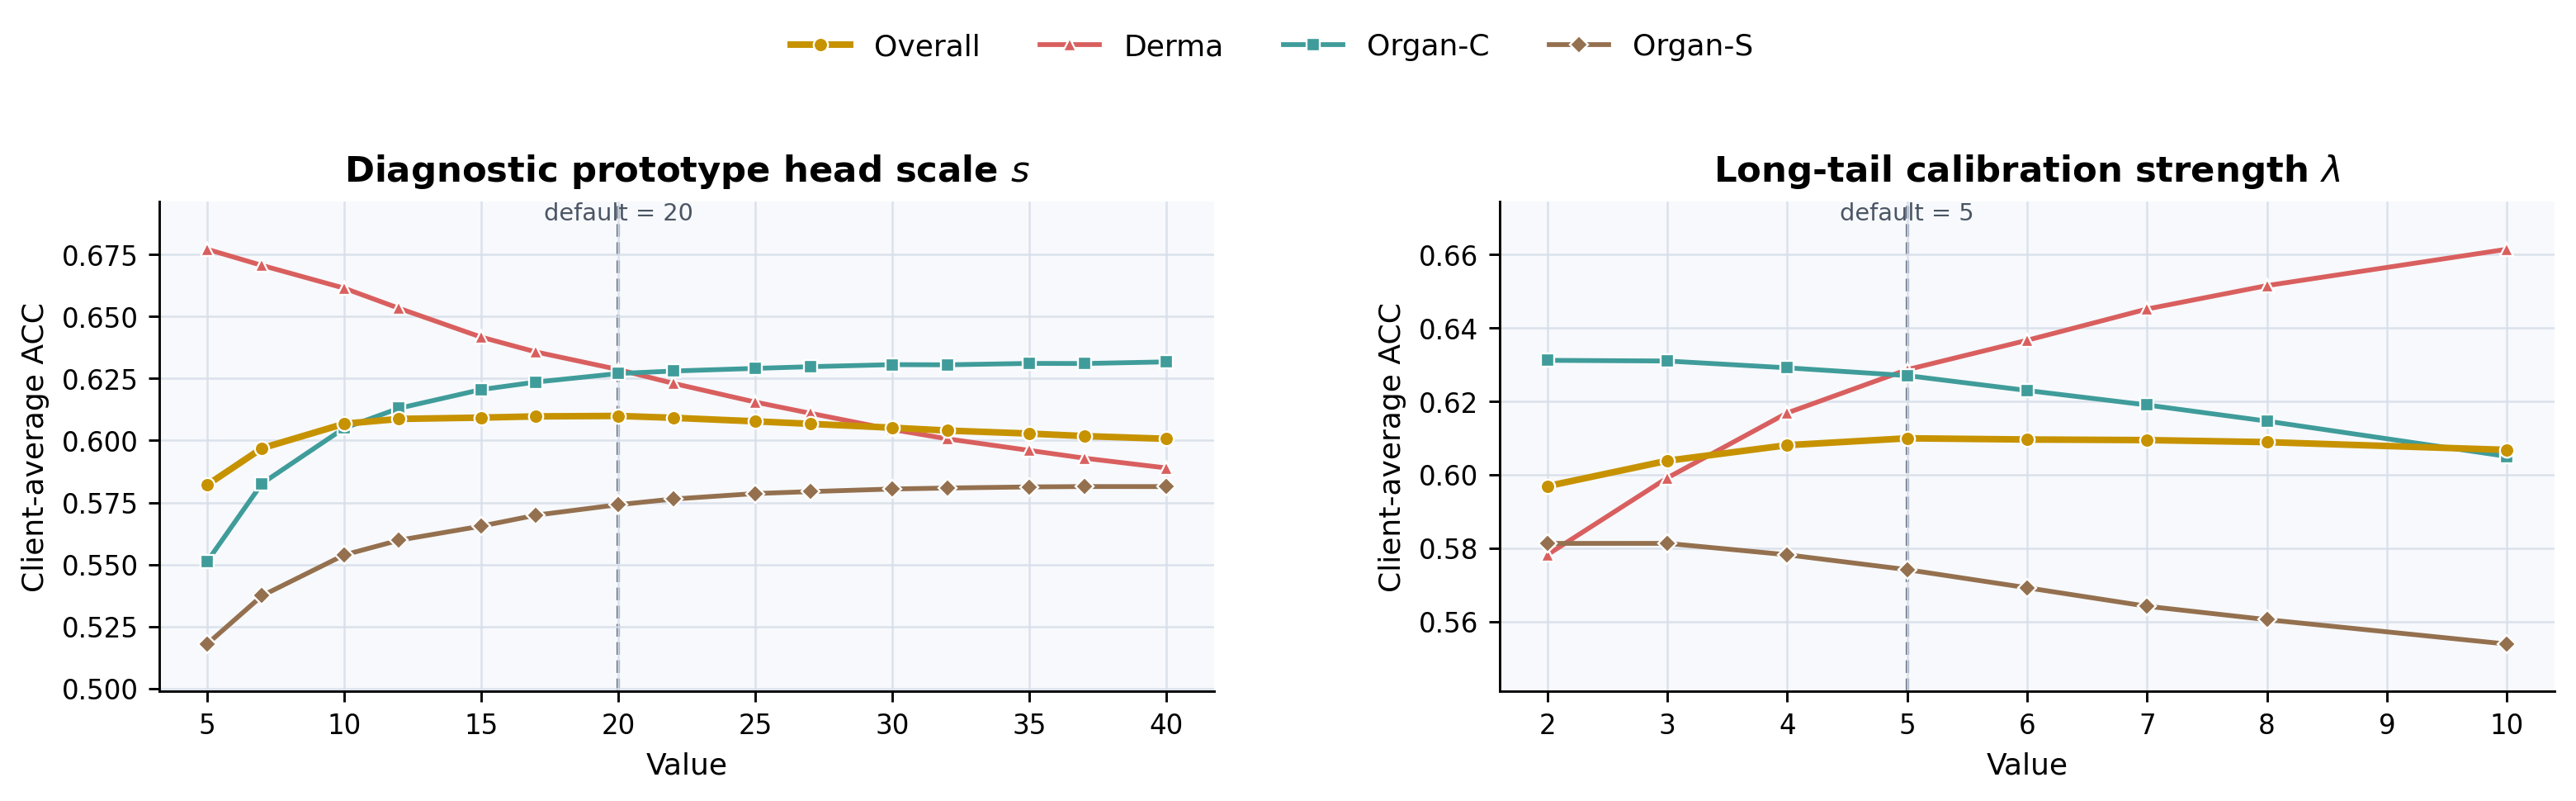
\includegraphics[width=0.92\textwidth]{figures/full_scope_hyperparameter_sensitivity.png}
\caption{Full-scope hyperparameter sensitivity with five fixed-value curves per module. The formal settings $s=20$ and $\lambda=5$ lie in stable high-accuracy regions.}
\label{fig:hparam-full}
\end{figure*}

% 结果说明，LAMP-Merge 在较宽的超参数范围内均保持稳定性能。原型头缩放因子 (s) 和长尾校准强度 (\lambda) 的变化只带来小幅波动，默认设置 (s=20,\lambda=5) 位于稳定高性能区间。因此我们的收益主要来自诊断原型重建与长尾患病率校准本身，而非依赖精细的超参数搜索。
For every fixed $\gamma$, the diagnostic-prototype curves attain their local maximum at $s=17.5$ or $s=20$ and decline only mildly at $s=25$. The formal $(\gamma,s)=(0.45,20)$ setting is within $0.0002$ of the maximum on its curve. Likewise, the formal $(\tau,\lambda)=(2.5,5.0)$ setting is within $0.0002$ of the maximum on its curve. Thus, the gain arises from the two components rather than narrow hyperparameter tuning.

\subsection{New-metric Diagnostic Experiment}
% 虽然主实验只用 ACC 进行横向比较，但医学长尾分布可能使单类或少数类预测器获得较高 ACC。因此，我们引入了新的指标。令 y_n 和 \hat y_n 分别表示第 n 个测试样本的真实标签和预测标签，令 q_c=N^{-1}\sum_n 1[\hat y_n=c] 表示预测类别分布，令 p_c=N^{-1}\sum_n 1[y_n=c] 表示真实类别分布，令 C_test 表示测试集中真实出现的类别集合。我们使用如下诊断指标。
Although the main experiments use ACC for direct comparison, long-tailed medical distributions can allow single-class or few-class predictors to achieve high ACC. We therefore introduce additional metrics. Let \(y_n\) and \(\hat{y}_n\) denote the true and predicted labels of the \(n\)-th test sample. Let \(q_c=N^{-1}\sum_n\mathbf{1}[\hat{y}_n=c]\) be the predicted-class distribution, \(p_c=N^{-1}\sum_n\mathbf{1}[y_n=c]\) be the true class distribution, and \(\mathcal{C}_{\mathrm{test}}=\{c\mid \sum_n\mathbf{1}[y_n=c]>0\}\) be the set of classes observed in the test set. We use the following diagnostic metrics.

\begin{itemize}
\item \(\mathrm{BA}=|\mathcal{C}_{\mathrm{test}}|^{-1}\sum_{c\in\mathcal{C}_{\mathrm{test}}}\mathrm{Recall}_c\). This is balanced accuracy, or macro recall, and measures whether all observed diagnosis classes are recalled.
\item \(\mathrm{MacroF1}=|\mathcal{C}_{\mathrm{test}}|^{-1}\sum_{c\in\mathcal{C}_{\mathrm{test}}}\mathrm{F1}_c\). This measures class-balanced precision-recall quality and penalizes methods that only preserve majority-class predictions.
\item \(\rho=\max_c q_c\). This is the prediction-collapse ratio and measures how strongly predictions concentrate on a single diagnosis class.
\item \(C_{\mathrm{eff}}=\exp\left(-\sum_c q_c\log q_c\right)\). This is the effective number of predicted classes and measures how many diagnosis classes are actually used by the model.
\item \(\mathrm{TV}(q,p)=\frac{1}{2}\sum_c |q_c-p_c|\). This is the total variation distance between predicted and true class distributions and measures whether the output distribution matches the test-set prevalence.
\end{itemize}


\begin{table}[t]
\centering
\caption{Prediction-collapse diagnostics averaged over five medical datasets and four backbones per dataset.}
\label{tab:collapse-key}
\scriptsize
\setlength{\tabcolsep}{2.5pt}
\renewcommand{\arraystretch}{0.92}
\begin{tabular}{lrcc}
\hline
\tblhead{Metric} & \metriclampcell{LAMP-Merge} & \tblhead{Best reference} & \tblhead{\(\Delta\) vs. LAMP} \\
\hline
Accuracy $\uparrow$ & \metriclampcell{0.6211} & 0.2228 & \gainup{+0.3983} \\
BA / macro recall $\uparrow$ & \metriclampcell{0.5370} & 0.1492 & \gainup{+0.3878} \\
Macro F1 $\uparrow$ & \metriclampcell{0.5238} & 0.0757 & \gainup{+0.4481} \\
Collapse ratio $\downarrow$ & \metriclampcell{0.3122} & 0.7902 & \gaindown{-0.4780} \\
Effective classes $\uparrow$ & \metriclampcell{7.1322} & 2.0489 & \gainup{+5.0833} \\
Pred-true TV $\downarrow$ & \metriclampcell{0.1262} & 0.7040 & \gaindown{-0.5778} \\
\hline
\end{tabular}
\end{table}

% 表*中将LAMP-Merge与各个指标的最高基线相对比。可以看到，该方法显著优于目前已有的算法。这说明 LAMP-Merge 的准确率提升并非来自更强的单类坍缩，而是来自更完整的全局诊断判别。
Table \ref{tab:collapse-key} compares LAMP-Merge with the best-performing baseline for each metric. LAMP-Merge consistently and substantially outperforms the existing methods. This indicates that its accuracy gains do not arise from more severe single-class prediction collapse, but rather from more complete global diagnostic discrimination.

\subsection{Visualization Experiment}

% 为了直观展示新指标诊断所反映的预测分布变化，我们进一步给出预测坍缩恢复图和代表性数据集上的预测类别分布图。
To visualize the prediction-distribution changes measured by the new diagnostic metrics, we provide a representative predicted-class distribution in Fig.~\ref{fig:visual-chaosheng_predict}.

\begin{figure}[t]
\centering
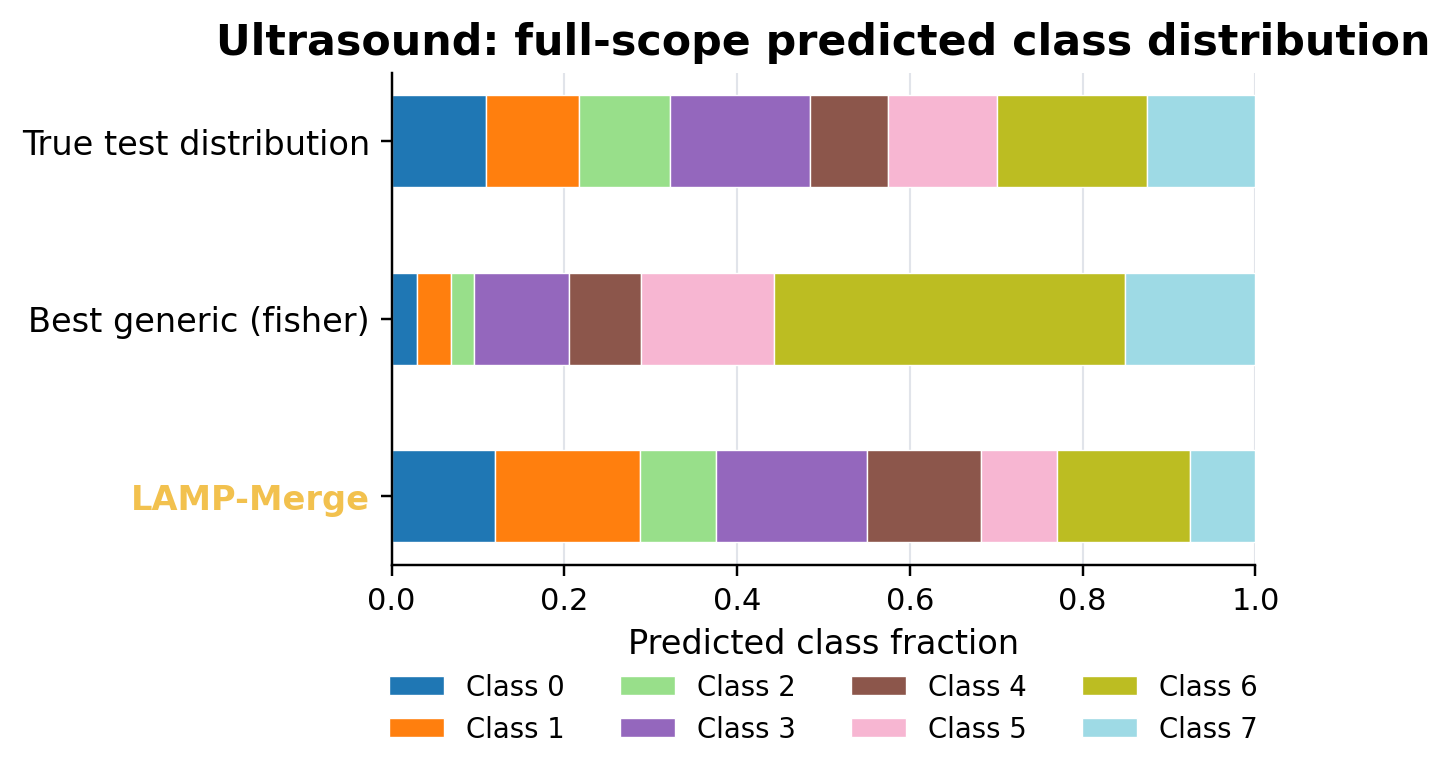
\includegraphics[width=\columnwidth]{figures/full_scope_predicted_distribution_ultrasound_stacked.png}
\caption{Predicted class distributions on Ultrasound, averaged over the four visual backbones, $K\in\{3,5,7\}$, and the three Dirichlet skew levels. The strongest generic reference (Fisher) concentrates predictions on a subset of classes, while LAMP-Merge recovers a broader allocation aligned with the test distribution.}
\label{fig:visual-chaosheng_predict}
\end{figure}

\subsection{t-SNE Visualization Experiment}
% 我们仅将 t-SNE 用于分析，而不用于服务器端选择或融合。图中给出了 Blood 数据集上 ResNet、K=3、beta=0.01 设置下的联合 t-SNE 对比。每个点对应一个测试图像的模型输出概率向量，不同正式融合方法在同一二维空间中投影，用于比较预测表征的类别结构。
We use t-SNE only for analysis, not for server-side selection or fusion. Fig.~\ref{fig:tsne} shows a joint comparison on Blood with ResNet, $K=3$, and $\beta=0.01$. Each point is the output-probability representation of a test image, and formal merging methods are projected into the same two-dimensional space to compare the class structure of their predictive representations.

\subsection{In-depth Analysis Experiment}
\subsubsection{1) analysis of the geometry}
% 最后，我们对诊断原型重建产生的几何结构进行深入分析。该实验对应模块内消融中的原型替换设置，用于解释为什么共享参考空间类别原型与类别级支持数共同带来稳定收益。令 d(a,b)=1-cos(a,b) 表示余弦距离，令 I_c 表示具有类别 c 样本的客户端集合。所用几何量定义如下。
Finally, we conduct an in-depth analysis of the geometry induced by diagnostic prototype reconstruction. This experiment corresponds to the prototype-replacement settings in the internal ablation and explains why reference-space class prototypes and class-level support counts jointly provide stable gains. Let \(d(a,b)=1-\cos(a,b)\) denote cosine distance, and let \(\mathcal{I}_c=\{i\mid n_{i,c}>0\}\) denote the set of clients that contain diagnosis class \(c\). The geometric quantities are defined as follows.

\begin{itemize}
\item \(D_{\mathrm{pair}}=\frac{2}{C(C-1)}\sum_{c<d}d(p_c,p_d)\). This is the mean distance between global prototypes of different diagnosis classes, measuring whether the reconstructed head forms separable class-level diagnostic directions.
\item \(D_{\mathrm{nn}}=\frac{1}{C}\sum_c \min_{d\ne c} d(p_c,p_d)\). This is the mean nearest-class distance, measuring the most vulnerable decision margin around each diagnosis prototype.
\item \(A_{\mathrm{client}}=\frac{1}{C}\sum_c \mathrm{Avg}_{i<j,\,i,j\in\mathcal{I}_c}\cos(\mu_{i,c},\mu_{j,c})\). This is the within-class consistency among client prototypes, measuring whether clients that observe the same diagnosis produce compatible evidence in the shared reference space.
\item \(A_{\mathrm{proto}}=\frac{1}{C}\sum_c\sum_{i\in\mathcal{I}_c}\alpha_{i,c}\cos(p_c,\mu_{i,c})\). This is the alignment between the server-side global prototype and the contributing client prototypes, measuring whether aggregation preserves client-side class evidence.
\end{itemize}

Fig.~\ref{fig:prototype-geometry} reports these four quantities for the controlled prototype substitutions in the internal ablation. The full method jointly preserves nonzero inter-class separation and high cross-client consistency and prototype-client alignment, rather than maximizing a single geometric value. Together with the accuracy drops in Table~\ref{tab:diagnostic-internal-ablation}, this joint profile shows that the benefit arises from class-semantic reference-space prototypes weighted by class-specific support.

\begin{figure*}[t]
\centering
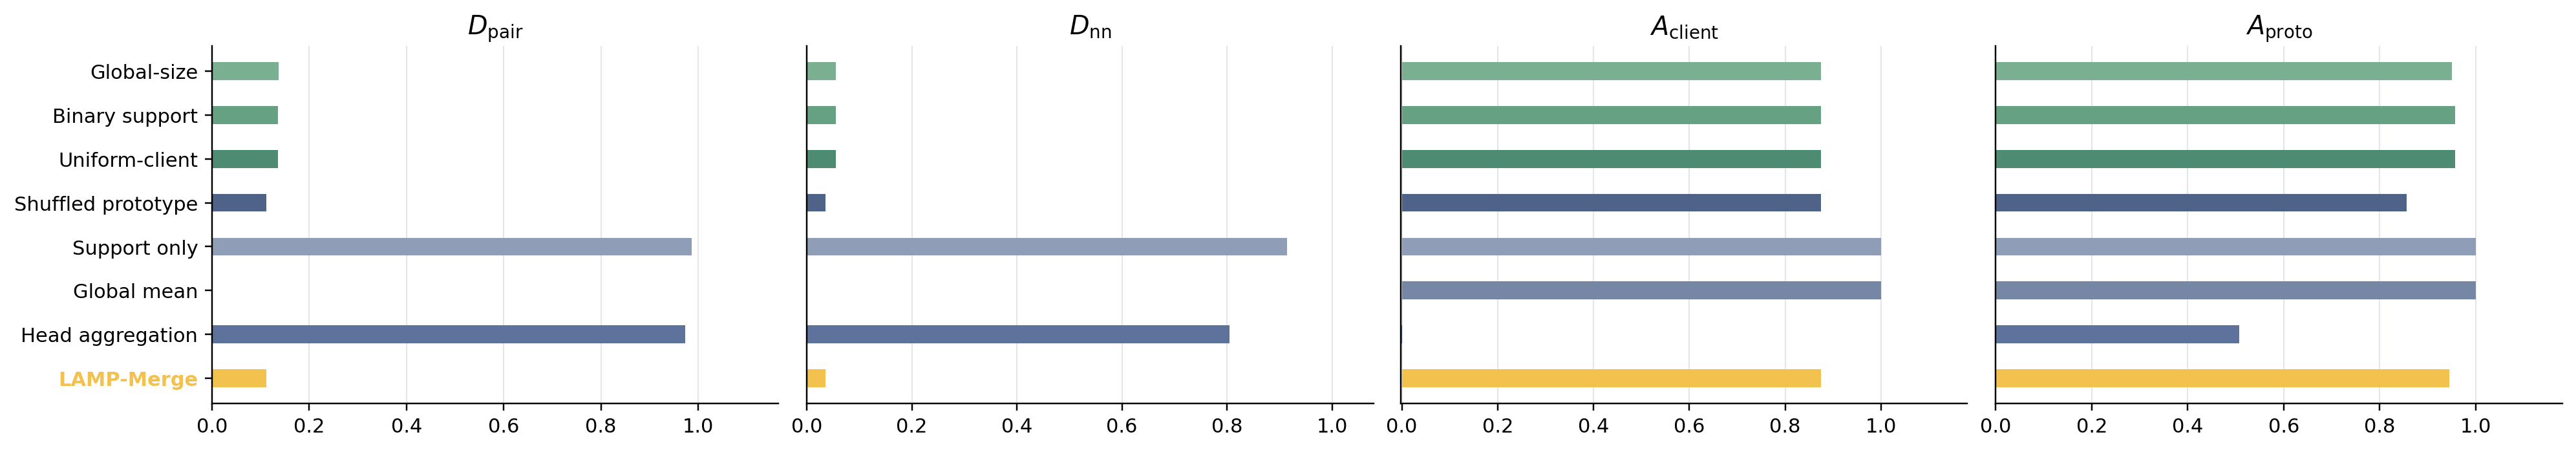
\includegraphics[width=0.96\textwidth]{figures/full_scope_prototype_geometry_internal_ablation.png}
% 完整基准上的原型几何比较。该图总结了两两距离、最近类别距离、原型一致性和原型-客户端对齐程度。
\caption{Prototype-geometry comparison on the full benchmark. The figure summarizes pairwise distance, nearest-class distance, prototype consistency, and prototype-client alignment.}
\label{fig:prototype-geometry}
\end{figure*}

The individual geometry values should therefore be interpreted as mechanism diagnostics, not standalone objectives: extreme separation or perfect alignment can be produced by class-agnostic or mismatched directions. LAMP-Merge is effective because its four quantities are simultaneously consistent with class semantics and the observed full-scope accuracy gains.

\subsubsection{2) Additional Theoretical Analysis}
% 令 mu_c^star 表示共享参考空间中的真实类别均值。如果客户端类别特征具有有界二阶矩，则原型估计误差满足如下上界。
Let $\mu_c^\star$ denote the true class mean in the shared reference space. If client class features have bounded second moments, the prototype estimation error satisfies
\begin{equation}
\mathrm{E}\|p_c-\mu_c^\star\|_2^2
\le
\sum_i \alpha_{i,c}^2\frac{\sigma_c^2}{n_{i,c}}
+ \mathrm{Bias}_c^2.
\end{equation}
% 该上界表明，支持数直接控制类别原型估计的方差。没有观测到类别 c 的客户端不应为该类别贡献证据；样本更多的客户端应贡献更多证据，但该贡献应是次线性的。
This upper bound shows that support counts directly control the variance of class-prototype estimation. A client that does not observe class $c$ should not contribute evidence for that class, and a client with more samples should contribute more, but only sublinearly.

% 令样本 x 在类别 c 和 d 之间的真实间隔为 Delta_c,d(x)。
Let the true margin between classes $c$ and $d$ for sample $x$ be
\begin{equation}
\Delta_{c,d}(x)=(\mu_c^\star)^\top z-(\mu_d^\star)^\top z.
\end{equation}
% 当原型误差满足下式时，估计原型能够保持类别 c 和类别 d 之间的排序。
When the prototype error satisfies
\begin{equation}
\|p_c-\mu_c^\star\|_2+\|p_d-\mu_d^\star\|_2
<
\frac{\Delta_{c,d}(x)}{\|z\|_2},
\end{equation}
the estimated prototypes preserve the class order between $c$ and $d$.

% 长尾患病率校准的作用是以有界方式引入长尾先验。对于患病率计数 m_i,c，类别先验为 pi_c，中心化对数先验偏置为 b_c。只要 lambda 有界，长尾患病率校准就不会替代诊断原型重建的判别方向；它只会将输出校准到真实类别患病率。这解释了为什么单独使用长尾患病率校准不充分，而完整 LAMP-Merge 能同时保持非坍缩性和患病率感知能力。
The role of long-tail prevalence calibration is to introduce long-tail priors in a bounded manner. For prevalence counts $m_{i,c}$, the class prior is
\begin{equation}
\pi_c=\frac{\sum_i m_{i,c}}{\sum_k \sum_i m_{i,k}},
\end{equation}
and the centered log-prior bias is
\begin{equation}
b_c=\lambda\left(\log\pi_c-\frac{1}{C}\sum_k\log\pi_k\right).
\end{equation}
As long as $\lambda$ is bounded, long-tail prevalence calibration does not replace the discriminative directions reconstructed by diagnostic prototype reconstruction; it only calibrates the output toward the real class prevalence. This explains why using long-tail prevalence calibration alone is insufficient, while full LAMP-Merge remains both non-collapsed and prevalence-aware.

\section{Conclusion}

% 本文研究了单次异步医学模型融合问题，其中独立训练的医院模型必须在没有联邦优化轮次且不向服务器暴露原始医学图像的条件下被融合。我们的实证分析表明，在局部诊断覆盖不完整时，通用模型融合方法会遭遇聚合诱导的预测坍缩。我们进一步表明，在长尾医学数据集上，这种坍缩可能被原始准确率掩盖，因此设计 Long-tail Prevalence Calibration模块并使用宏召回率、宏 F1 和预测分布诊断进行二次评估。
We studied one-shot asynchronous medical model merging, where independently trained hospital models must be fused without federated optimization rounds and without exposing raw medical images to the server. Our empirical analysis shows that generic model-merging methods suffer from aggregation-induced predictive collapse under incomplete local diagnostic coverage. We further show that, on long-tailed medical datasets, such collapse can be masked by raw accuracy. We therefore introduce the Long-tail Prevalence Calibration module and perform secondary evaluation using macro recall, macro-F1, and predictive-distribution diagnostics\cite{BUDA2018249,5597285}.

% LAMP-Merge 以简洁的双模块设计处理这两个性质。未来我们将进一步扩展 LAMP-Merge 的适用范围：一方面，将其从医学图像分类拓展到分割、检测及多模态诊断任务；另一方面，研究更严格的隐私保护机制，例如差分隐私或安全聚合，以进一步降低类别级统计信息可能带来的隐私风险。同时，我们也将探索在更大规模真实多中心医疗场景中的部署与验证。
LAMP-Merge addresses these two properties through a concise two-module design. Future work will extend its applicability in two directions: first, from medical image classification to segmentation, detection, and multimodal diagnostic tasks; and second, toward stronger privacy-preserving mechanisms, such as differential privacy and secure aggregation, to further reduce potential privacy risks associated with class-level statistics\cite{kaissis2020secure,geyer2017differentially,abadi2016deep}. We will also explore deployment and validation in larger-scale real-world multicenter healthcare settings.


\bibliography{aaai2026}
\end{document}
